\chapter{Математичні основи теорії кодів автентифікації}
\minitoc

\section{Лекція 1. Автентифікація. Сценарії загроз автентифікації. Підходи до забезпечення цілісності і автентичності.}

\subsection{Вступ}

У курсі розглядаються загальні підходи до автентифікації повідомлень,
теоретичні поняття кодів автентифікації їх властивості, алгоритми побудови
стійких кодів автентифікації, можливі атаки на автентичність і способи
захисту від них, а також аспекти практичного застосування цих питань до
проблем побудови, застосування і оцінювання стійкості кодів
автентифікації.

% \textbf{Зміст навчальної дисципліни}

% \begin{enumerate}
%     \item Розділ 1. Поняття автентичності повідомлення. Загальні підходи до автентифікації повідомлень.
%     \begin{enumerate}
%         \item Тема 1.1. Цілісність інформації та автентифікація. Моделі і сценарії загроз автентифікації.
%             Підходи до забезпечення цілісності і автентичності.
%         \item Тема 1.2. Учасники систем автентифікації. Криптографія та коди автентифікації. Приклади кодів автентифікації.
%         \item Тема 1.3. Поняття автентичності повідомлення. Імітостійкість за
%         Сіммонсом.
%     \end{enumerate}
%     \item Розділ 2. Математичне визначення коду автентифікації ($A$-коду).
%     Характеристики $A$-кодів.
%     \begin{enumerate}
%         \item Тема 2.1. Загальне визначення коду автентифікації. $A$-коди з
%         секретністю і без секретності. Параметри та характеристики $A$-кодів.
%         Порівняння $A$-кодів та криптографічних систем шифрування.
%         \item Тема 2.2. Умови на параметри $A$-кодів. Матриці $A$-коду, інцидентності,
%         табличного задання $A$-коду.
%         \item Тема 2.3. Перевірка обов'язкових умов. Можливі атаки на
%         автентичність повідомлення при порушенні окремих умов. Приклади
%         $A$-кодів та можливих атак.
%     \end{enumerate}
%     \item Розділ 3. Декартові $A$-коди без секретності.
%     \begin{enumerate}
%         \item Тема 3.1. Декартові $A$-коди без секретності та $A$-коди з
%         автентифікатором. Побудова $A$-коду з автентифікатором за матрицею
%         $A$-коду. Матриця автентифікації $A$-коду з автентифікатором.
%         \item Тема 3.2. Приклади побудови $A$-коду з автентифікатором за матрицею
%         $A$-коду та атак на автентичність повідомлення.
%         \item Тема 3.3. Алгебраїчно-ймовірнісна модель $A$-коду. Безумовно стійкі $A$-коди.
%             Методи побудови безумовно стійких $A$-кодів без секретності.
%     \end{enumerate}
%     \item Розділ 4. Безумовно стійкі $A$-коди з секретністю.
%     \begin{enumerate}
%         \item Тема 4.1. Безумовно стійкі $A$-коди з секретністю. Методи побудови.
%         \item Тема 4.2. Приклади побудови $A$-кодів з секретністю. Приклад $A^2$-коду і
%         можливих атак на автентичність.
%     \end{enumerate}
% \end{enumerate}

\subsection{1.1. Цілісність інформації та автентифікація. Моделі і сценарії загроз.}

Основними задачами теорії \textbf{імітостійкості і автентичності} є
забезпечення цілісності та справжності інформації і джерела інформації та
інформаційних ресурсів.

\textbf{Цілісність інформації та інформаційних ресурсів} -- це властивість
захищеності інформації від випадкової чи навмисної її модифікації, яка
забезпечується за рахунок застосування криптографічного перетворення
інформації.

\textbf{Автентифікація повідомлень} -- це процедура перевірки цілісності і
справжності повідомлення, отриманого від визначеного об'єкта.

\textbf{Автентифікація інформації} -- це процедура перевірки цілісності цієї інформації,
якщо вона протягом деякого часу знаходилась поза контролем власника і підтвердження авторства цієї інформації.

\textbf{Автентифікація джерела (автора) інформації} -- це процедура
підтвердження, у тому числі і юридично, того факту, що інформація створена
або відправлена певним об'єктом чи суб'єктом.

\textbf{Ідентифікація} -- це процедура присвоєння об'єктам, суб'єктам чи
процесам унікального імені чи коду, наявність якого дозволяє однозначно
виділити цей об'єкт чи процес серед інших.

\textbf{Автентифікація користувача} -- це певна процедура встановлення дійсності об'єкта чи
суб'єкта, що звертається до інформації чи ресурсів, що захищаються.

\textbf{Автентифікація мережі} -- це процедура встановлення дійсності та
справжності мережі чи інформаційної технології, до яких отримується доступ
даним об'єктом чи суб'єктом.

\textbf{Невідмовність отримувача} -- це процедура підтвердження, у тому числі і
юридично, факту прийому й обробки об'єктом чи суб'єктом конкретної
інформації.

\textbf{Невідмовність відправника} -- це процедура підтвердження, у тому числі і
юридично, факту обробки й відправлення об'єктом чи суб'єктом конкретної
інформації.

\textbf{Спостережливість} -- це властивість, що є показником захищеності інформації і ресурсів
комп’ютера, комп'ютерної мережі, АСУ і т. д., що забезпечує реєстрацію і
спостереження за діями й автентифікацію усіх об'єктів процесу, відстеження
небезпечних дій, попередження чи обмеження користувачів процесів,
насамперед за рахунок криптографічного захисту інформації.

\textit{Автентифікація} здійснюється за рахунок застосування систем
паролювання, кодів автентифікації системи, електронних підписів та
електронних цифрових підписів.

Моделі і сценарії загроз автентичності.

На рис. \ref{fig:enter_label1} наведена спрощена схема моделі взаємної недовіри і
взаємного захисту.

\begin{figure}
    \centering
    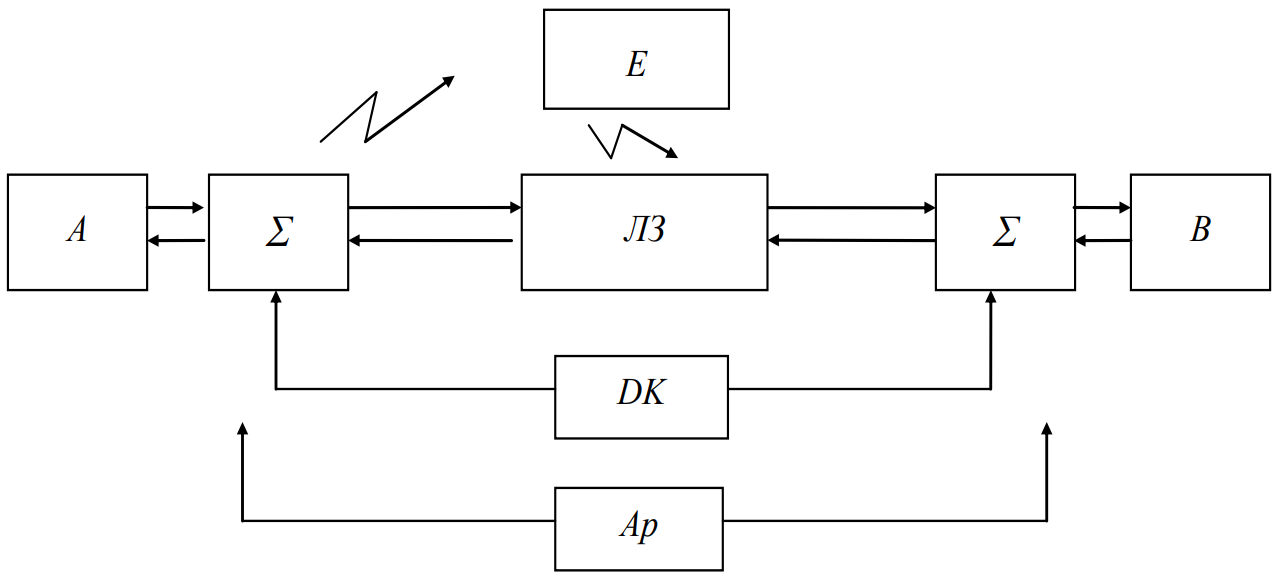
\includegraphics[width=0.5\linewidth]{Images/image1.png}
    \caption{Спрощена схема моделі взаємної недовіри і взаємного захисту}
    \label{fig:enter_label1}
\end{figure}

На рис. \ref{fig:enter_label1} позначено:
\begin{itemize}
    \item $A$, $B$ – користувачі, джерела інформації;
    \item $\Sigma$ – засіб захисту інформації;
    \item ЛЗ – телекомунікаційна система (носій інформації);
    \item $E$– криптоаналітик (зловмисник);
    \item ДК – джерело ключів;
    \item Ар – арбітр.
\end{itemize}

Суб'єкти $A$, $B$, $E$, Ар не довірять один одному і можуть робити спроби з
метою обману інших. Атаки с порушенням цілісності та автентичності
вважаються успішними, якщо отримувач не розпізнав дезінформації і прийняв
надіслане повідомлення як справжнє. Ймовірність успіху є однією з головних
характеристик небезпеки таких атак дезінформації. Розглянемо деякі сценарії і
класи атак порушення цілісності та автентичності, які можуть бути реалізовані
суб'єктами $A$, $B$, $E$, Ар.

Основні загрози, що може реалізувати джерело А, яке передає повідомлення:
\begin{enumerate}
    \item джерело $A$ формує повідомлення $M_i$, а потім відмовляється від факту передачі його в мережу;
    \item джерело $A$ стверджує, що він сформував деяку інформацію $M_i$ і передав у мережу,
        а насправді він її не формував і не передавав;
    \item $A$ стверджує, що він сформував і передав інформацію $M_i$ у визначений
        час, хоча насправді він її сформував і передав іншим часом;
    \item $A$ формує і передає інформацію $M_i'$, а потім стверджує, що була
        передана інформація $M_i$.
    \item тощо.
\end{enumerate}

Основні загрози, що може реалізувати отримувач джерело В у спробі обманути A:
\begin{enumerate}
    \item $B$ сам формує деяку $M_i'$ інформацію, а потім $B$ стверджує, що він її
        отримав від $A$;
    \item $B$ отримує $M_i$ інформацію від $A$, модифікує її в $M_i'$ , а потім стверджує,
        що він отримав цю інформацію від $A$;
    \item $B$ стверджує, що він отримав інформацію $M_i$ в момент часу $t_i$, а
        насправді він отримав інформацію під час $t_j$;
    \item $B$ отримує інформацію $M_i$, а потім стверджує, що він її не отримав;
    \item Тощо.
\end{enumerate}

Основні загрози, що може реалізувати криптоаналітик E:
\begin{enumerate}
    \item імітація помилкового повідомлення $M_i$: $E$ у момент часу, коли $A$
        пасивний, створює помилкову інформацію $M_i$ і передає її $B$;
    \item модифікація правильної інформації $M_i$, у випадку, якщо $A$ передає $B$,
    деяку інформацію $M_i$, $E$ модифікує інформацію $M_i$ в $M_i'$ і передає її $B$;
    \item нав'язування раніше створеної інформації, тобто $E$ в будь-який
        момент часу $t_j$ передає її ще раз $B$, коли $A$ пасивний;
    \item передача хибних команд керування мережними службами,
        помилкові команди керування ключами, підміна сертифікатів тощо.
\end{enumerate}

Арбітра Ар також можна вважати зловмисником і не довіряти йому, від
нього потрібно також захищатися. Арбітр Ар може для атак використовувати
додаткову привілейовану інформацію і значно підвищити ймовірність успішної
дезінформації.

Основні загрози, що може реалізувати арбітр Ар:
\begin{enumerate}
    \item якщо арбітр Ар не має доступу до привілейованої інформації, тоді у Ар такі
        ж можливості і реалізації загроз, як у криптоаналітика $E$;
    \item арбітр Ар, використовуючи як відкриту інформацію, так і свою
        привілейовану, формує фальшиве повідомлення $M_i$ і відправляє $B$;
    \item Ар чекає і перехоплює повідомлення від $A$ ($B$), потім, використовуючи свою
        додаткову привілейовану інформацію і аналіз перехопленого повідомлення,
        формує хибне повідомлення і відправляє його $B$ ($A$).
\end{enumerate}

Якщо в системах з телекомунікаційним зв’язком виконується багатократний
обмін інформаційними повідомленнями, то для порушенням цілісності та
автентичності можлива низка різних сценаріїв і атак дезінформації. Наприклад:
модифікація послідовності повідомлень, виключення деяких або зміна порядку
слідування повідомлень, зміна часових характеристик, заміна деяких повідомлень
раніш надісланими тощо. Існує багато наукових робіт Г. Сіммонса та інших
фахівців, в яких досліджувалися характеристики таких атак та способи захисту від
них.

\begin{example}
    Приклад 1.1. Нехай повідомлення $M$, що передається в банк, складається з
    одного блоку зі 128 біт, в якому міститься інформація про переказ певної суми з
    однієї карти на іншу. З метою автентифікації повідомлення $M$ зашифровується
    потоковим шифром гамування з використанням секретного ключа (або блоковим
    в режимі зворотного зв’язку за виходом чи в режимі лічильника): $C = E_k(M)$.
    Нехай останні 16 біт виділено для запису суми переводу в двійковому вигляді.
    Припустимо, що сума переказу 200 у.о., або 0000000011001000. Зловмисник
    (наприклад, отримувач, який знає очікувану суму) може виконати атаку підміни
    на ШТ зі зміною суми:
    $$\Tilde{C} = C \oplus 0^{12}0000011100001000$$
    Після розшифрування $D_k(\Tilde{C}) = \Tilde{M}$ у ВТ зміниться тільки сума і банк
    для переказу отримує суму
    
    $$0000000011001000 \oplus 0000011100001000 = 0000011111001000 =
    2000 \text{у.о.}$$
    При цьому, не зважаючи на шифрування, банк по формату і змісту
    розшифрованого повідомлення не може виявити підробки. Аналогічно, якщо
    відомі в блоці повідомлення позиції картки отримувача і її номер, може бути
    проведена атака підміни з переказом на інший рахунок.
\end{example}

\subsection{1.2. Підходи до створення способів перевірки і підтвердження цілісності і автентичності повідомлень.}

Які існують можливості в забезпеченні надійного підтвердження
справжності або автентичності повідомлень або файлів, що зберігаються.
Головним напрямом у підходах побудови систем підтвердження цілісності і
автентичності є структуризація, створення і додавання до повідомлення
спеціальної додаткової інформації та надлишковості. Розглянемо приклади.

1. Простіший метод перевірки цілісності файлів полягає в обчисленні
його контрольної суми, яка зберігається в захищеному від зловмисника місті.
Для перевірки власник файлу знову обчислює контрольну суму і порівнює
результати з вихідною контрольною сумою. Незбіг контрольних сум свідчить
про порушення цілісності.

У якості контрольної суми зручно використовувати односторонні сильні
хеш-функції (безключові), які, зазвичай, називають кодом розпізнавання
помилок. Якщо передається повідомлення по незахищеному каналу, то
контрольна сума повинна передаватися по окремому каналу з підтвердженням.

Якщо зловмиснику відомий спосіб обчислення контрольної суми, то він
може відправити фальшиве повідомлення з правильною контрольною сумою,
які отримувачем буде прийнято за достовірне. Зберігати ж у секреті повний
спосіб обчислення контрольної суми і передавати такий секрет по закритому
каналу дуже непрактичні і ненадійні процедури. Тут можна використовувати
секретні ключи.

2. Одним зі способів забезпечити цілісність у цьому випадку є
використання секретної інформації (ключа) у відправника і отримувача та
шифрування змістовної інформації, яка має значну надлишковість і достатньо
надійно може бути перевірена статистичними тестами на відкритий текст. В
цьому випадку, як випливає з теорії імітостійкості Симмонса, ймовірність
обману при випадковому виборі ШТ для абсолютно імітостійкої криптосистеми
$P_{\text{обм.}} = \frac{|\mathfrak{M}|}{|\mathfrak{C}|}$
і може бути зроблена знехтовно малою. Цей спосіб для
забезпечення надійності при практичному використанні повинен мати низку
застережень.

3. Іншим способом забезпечити цілісність у цьому випадку є
використання секретної інформації (ключа) у відправника і отримувача, з
використанням якої відбувається обчислення контрольної суми. В системі
користувачів, які довіряють один одному і мають спільний секретний ключ, тут
може використовуватися хеш-функція зі спільним секретним ключем або
безключова функція з окремим «замішуванням» в контрольну суму інформації
з секретного ключа.

4. Використання симетричної системи шифрування з секретним ключем,
наприклад, в режимі зчеплення блоків для вироблення імітовставки, яка
додається до повідомлення і має за мету саме підтвердження його цілісності.
Такий спосіб (як і використання хеш-функція з секретним ключем) дає
можливість не тільки перевірити цілісність повідомлення, а й автентифікувати
відправника як учасника системи користувачів зі спільним секретним ключем.
Перевірка цілісності при використанні хеш-функція з секретним ключем або
імітовставки в режимі зчеплення блоків можливо і без шифрування ВТ
повідомлення, якщо в цьому немає потреби. Але в таких системах власники
секретного ключа мають можливість обманути один одного.

5. Обчислення контрольної суми повідомлення з допомогою деякої
функції F, яка додається до повідомлення і зашифровується симетричною
криптосистемою – так званий внутрішній контроль помилок.

6. Інший спосіб. Спочатку виконується шифрування, а потім
обчислюється функція F (контрольна сума) і значення додається до ШТ - так
званий зовнішній контроль помилок. При цьому якщо функція F відома
криптоаналітику, то він може створювати фальшиві шифротексти з
правильними контрольними сумами.

7. Опишемо один з прийнятих в США військових протоколів
автентифікації. Учасники $A$ і $B$ мають впорядкований (пронумерований) набір
секретних випадкових послідовностей фіксованої довжини $r$ (кожна в
окремому запечатаному конверті). Відправник додає до ВТ першу не
використану послідовність, шифрує симетричною системою на спільному
ключі і відправляє отримувачу. Отримувач розшифровує ШТ бере таку ж
послідовність у відповідному конверті та звіряє з останніми $r$ бітами
розшифрованого тексту. Якщо має місце збіг усіх $r$ бітів послідовності, то
автентифікація підтверджена. Ймовірність обману тут не більше $2^{-r}$.

В середовищі користувачів, які не довіряють один одному, використання
цифрового підпису в асиметричних криптосистемах дає можливість
забезпечити надійне підтвердження не тільки цілісності, а й автора (джерела)
повідомлення. Але для багатьох застосувань цифровий підпис не є достатньо
ефективним інструментом. Наприклад, для коротких повідомлень, які
використовуються в смарт-картах виробка цифрового підпису і його перевірка
потребують значного часу. Крім того, для зберігання заголовку цифрового
підпису, довгих асиметричних ключів і системних параметрів потрібно
значний об’єм пам’яті. Це робіть менш ефективним використання
асиметричних криптосистем для автентифікації і суттєво ускладнює
використання їх в малоресурсних криптографічних інструментах. По цим
причинам в середовищі користувачів, які довіряють один одному,
інформаційний обмін для перевірки цілісності і автентифікації виконується
симетричними алгоритмами шифрування. Симетричне шифрування може
використовуватись і в середовищі користувачів, які не довіряють один одному,
з залученням ще одного учасника – арбітра, якому довіряють інші учасники.
Але може статись, що арбітр теж може бути порушником в системі.

Важливою позитивною якістю застосування симетричних криптосистем є
висока швидкодія, можливість створити безумовно стійкі системи перевірки
цілісності і автентифікації. Розробка безумовно стійких систем автентифікації
почалася в середині 70-х років минулого століття під керівництвом
Г.Симмонса. Як ми бачили в теорії імітостійкості і в прикладі 1.1 шифрування
не забезпечує автоматично цілісність і автентичність інформації разом з її
конфіденціальністю. В загальному випадку криптографічна стійкість і
імітостійкість є незалежними властивостями системи захисту. 


\section{Лекція 2. Математична модель криптосистеми сформована Шенноном. Імітостійкість за Сіммонсом.}

\subsection{2.1. Алгебраїчно-ймовірнісна модель криптосистеми за Шенноном.}

При побудові теорії імітостійкості один з перших розробників в середині
70-х років минулого століття Г.Сіммонса спирався на алгебраїчно-ймовірнісну
модель криптосистеми Шеннона. Нагадаємо основні положення теорії
секретних систем Шеннона.

З математичної точки зору криптосистема є сукупністю просторів (множин) 
\begin{equation*}
    \Sigma = \{\mathbf{M}, \mathbf{K}, \mathbf{C}, \mathbf{E}, \mathbf{D}\},
\end{equation*}
де:
\begin{itemize}
    \item $\mathbf{M}$ - простір всіх повідомлень;
    \item $\mathbf{K}$ - простір ключів;
    \item $\mathbf{C}$ - простір криптограм;
    \item $\mathbf{E}$ - простір алгоритмів шифрування;
    \item $\mathbf{D}$ - простір алгоритмів розшифрування.
\end{itemize}


Розглянемо $M, X \in \mathbf{M}$ - деякі повідомлення, звичайно повідомлення - це
послідовність букв деякого алфавіту: $M = (m_1, m_2, ..., m_n)$, $X = (x_1, x_2, ..., x_n)$, $m_i$, $x_i$
-- символи ВТ, що є буквами відповідного алфавіту;
$C, Y \in \mathbf{C}$ -- криптограми, що
теж є, як правило, послідовністю символів деякого алфавіту;
$k \in \mathbf{K}$ -- деякий ключ;
$E_k \in \mathbf{E}$, $D_k \in \mathbf{D}$ -- конкретні перетворення (алгоритми) шифрування і
розшифрування з ключем $k$.
У загальному випадку шифр -- це відображення $\mathbf{M} \times \mathbf{K} \rightarrow \mathbf{C}$ таке, що виконуються співвідношення
$$\forall k \in \mathbf{K}, M \in \mathbf{M}: \quad D_k(E_k(M)) = M,$$
де $E_k: \mathbf{M} \rightarrow \mathbf{C}$ -- ін'єктивне відображення, що дає можливість зашифрувати
будь-який ВТ на ключі $k$. Ця властивість шифру називається однозначністю
розшифрування. Перед початком секретного зв’язку, як правило, один з
користувачів випадково генерує секретний ключ і передає іншому по закритому
каналу.

\begin{figure}
    \centering
    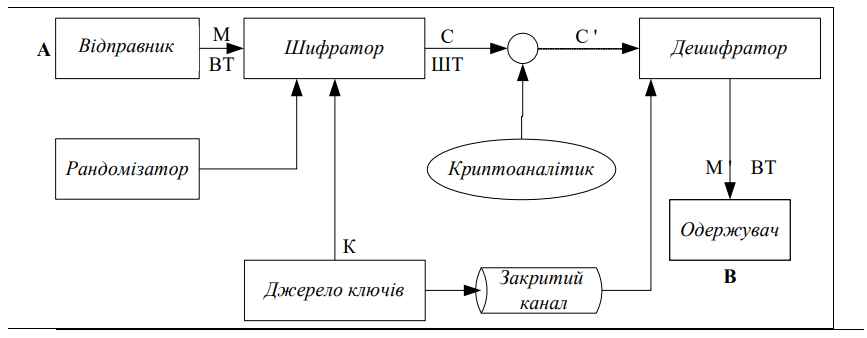
\includegraphics[width=0.5\linewidth]{Images/Secret_comunication_general_scheme.png}
    \caption{Загальна схема секретного зв'язку.}
    \label{fig:enter-label}
\end{figure}

В теорії Шеннона сформульовані наступні припущення:
\begin{enumerate}
    \item Криптоаналітику відомий тільки шифрований текст, тобто атака здійснюється на основі шифротексту.
    \item Ключ і рандомізатор використовуються для шифрування тільки один раз (тобто криптоаналіз здійснюється тільки по одній криптограмі).
    \item 3. На декартовому добутку $\mathbf{M} \times \mathbf{K}$ задано ймовірнісний розподіл.
\end{enumerate}

Цей список може бути доповнений новими припущеннями, які Шеннон
використовував неявно, зокрема, такими: канал передачі без спотворень,
перетворення інформації без помилок, відсутній зворотний зв’язок. Хоча вже
розроблені більш загальні теорії, результати Шеннона заклали наріжний камінь
криптографії як науки.

Побудова ймовірнісних розподілів і сумісних розподілів на інших множинах криптосистеми $\Sigma = \{\mathbf{M}, \mathbf{K}, \mathbf{C}, \mathbf{E}, \mathbf{D}\}$.

Згідно з правилом Керкгоффса всі простори криптосистеми $\Sigma$ та розподіл на $\mathbf{M} \times \mathbf{K}$ вважаються відомими криптоаналітику.

Нехай $P(M, k)$, $\sum\limits_{M, k} P(M, k) = 1$. -- розподіл імовірностей на декартовому
добутку $\mathbf{M} \times \mathbf{K}$. Зокрема, якщо відкритий текст і ключ, що генеруються,
незалежні (а частіше всього саме так на практиці), то $P(M, k) = P(M) \cdot P(k)$
Цей розподіл $P(M, k)$ індукує розподіли ймовірностей на інших множинах
системи.

\begin{enumerate}
    \item На просторах алгоритмів шифрування $\mathbf{E}$, алгоритмів розшифрування $\mathbf{D}$ та
    просторі криптограм $\mathbf{C}$ розподіли задаються формулами:
    $$\forall (k) \quad P(E_k) = P(D_k) = P(k),$$
    $$\forall (C) P(C) = \sum\limits_{\forall (M, k) \in \mathbf{M} \times \mathbf{K}: E_k(M) = C} P(M, k),$$
    де останнє підсумовування здійснюється за правилом суми ймовірностей
    несумісних подій по всіх парах $(M, k)$, для яких $E_k(M) = C$.
    \item Сумісний розподіл ймовірностей криптограм і ключів на декартовому
    добутку $\mathbf{C} \times \mathbf{K}$ задається формулою:
    $$\forall (C, k) \quad P(C, k) = \sum\limits_{\forall M \in \mathbf{M}: E_k(M) = C} P(M, k).$$
    \item Сумісний розподіл ймовірностей криптограм і відкритих текстів на $\mathbf{C} \times \mathbf{M}$ індукується наступними співвідношеннями:
    $$\forall (C, M) \quad P(C, M) = P(M, C) = \sum\limits_{\forall k \in \mathbf{K}: E_k(M) = C} P(M, k).$$
    \item Ймовірнісні розподіли на вказаних декартових добутках дають можливість
    знайти умовні розподіли:
    $$P(M | C) = \frac{P(M, C)}{P(C)}, P(C | M) = \frac{P(M, C)}{P(M)}, P(k | C) = \frac{P(k, C)}{P(C)}.$$
\end{enumerate}

\begin{definition}[Цілком таємна криптосистема]
    Цілком таємною криптосистемою $\Sigma$ називається
    криптосистема, для якої виконується одна з умов:
    \begin{enumerate}
        \item $(\forall M, C): P(M | C) = P(M)$;
        \item $H(\mathbf{M} | \mathbf{C}) = H(\mathbf{M})$, де $H(\mathbf{M})$ і $H(\mathbf{M} | \mathbf{C})$-- ентропія і умовна ентропія відповідно.
    \end{enumerate}
\end{definition}

\begin{remark}
    Умови 1 і 2 еквівалентні, з виконанням однієї умови буде
    виконуватись і інша. Умова 1 означає, що ВТ і ШТ статистично незалежні.
    Умову 2 можна інтерпретувати як відсутність в ШТ інформації відносно ВТ,
    тобто взаємна інформація
    $I(\mathbf{M}, \mathbf{C}) = H(\mathbf{M}) - H(\mathbf{M} | \mathbf{C}) = 0.$
\end{remark}

\subsection{1.1. Теорія імітостійкості Сіммонса.}

Ранiше вважалося, що якщо зашифрували вiдкритий текст, шифрований
текст вiдправили законному користувачевi та йому вдалось розшифрувати його,
то відкритий текст є цiлiсним. Але це виявляється не зовсiм так. Теорiю
імітостійкості на зразок теорiї Шеннона в 80-х роках XX століття розвинув
Г.Сіммонс. В алгебраїчно-ймовірнісній моделі Шеннона Симмонс розглянув
типи атак на цілісність повідомлень, коли атака криптоаналiтика E
здiйснюється за допомогою шифротексту: атака імітації, атака підміни і атака
обману.

\begin{enumerate}
    \item Атака імітації.
    Криптоаналітик $E$, не чекаючи повідомлення (ШТ) С від $A$, формує і
    відправляє $B$ хибний ШТ $\Tilde{C}$, $\Tilde{C} \rightarrow B$.
    Спроба імітації вважаеться успішною, якщо $B$ не розпізнав, що криптограма
    хибна і прийняв $\Tilde{C}$ за допустимий ШТ від $A$.
    $E$, знаючи ймовірнісні розподіли в моделі Шеннона, вибирає ШТ, який
    максимізує ймовірність успіху імітації
    $$P_{\text{ім.}} = \max\limits_{\Tilde{C} \in \textbf{C}} P(\Tilde{C} \text{-- допустима}).$$
    \item Атака підміни.
    Криптоаналітик $E$, після перехоплення від $A$ ШТ $C$, формує і відправляє $B$
    хибну криптограму $\Tilde{C}$, $\Tilde{C} \neq C$, $\Tilde{C} \rightarrow B$. Спроба підміни вважається успішною,
    якщо $B$ прийняв $\Tilde{C}$ за допустиму (від $A$), навіть якщо $B$ пізніше отримав
    істинну криптограму $\Tilde{C}$.

    Ймовірність успіху підміни $E$ максимізує вибором $\Tilde{C}$, розраховуючи
    ймовірності за моделлю Шеннона,
    $$P_{\text{підм.}} = \max\limits_{\Tilde{C} \in \mathbf{C}, \Tilde{C} \neq C} P(\Tilde{C} \text{-- допустима}).$$
    \item Атака обману. Криптоаналітик Е, знаючи ймовірнісні розподіли в моделі
    Шеннона, знаходить ймовірності $P_{\text{ім.}}$ і $P_{\text{підм.}}$
    і для обману $B$ використовує атаку з більшою ймовірністю успіху. Позначимо ймовірність такого обману
    $$P_{\text{обм.}} = \max\{P_{\text{ім.}}, P_{\text{зам.}}.$$
\end{enumerate}

Позначимо множину всіх можливих ШТ при роботі $A$ і $B$ на ключі $k$
через $\mathbf{C}_{k_i}$. Із-за однозначності розшифрування випливає:
$$(\forall k_i \in \mathbf{K}): |\mathbf{C}_{k_i}| \geqslant |\mathbf{M}|$$
При випадковому виборі ключа $k$ абонентами $A$ і $B$ і випадковому виборі
$\Tilde{C}$ криптоаналітиком, ймовірність імітації
\begin{equation}\label{eq:rand_choise}
    P_{ \text{ім.}} = \frac{|\textbf{C}_k|}{|\textbf{C}|} \geqslant \frac{|\textbf{M}|}{|\textbf{C}|}.
\end{equation}

Тобто, $P_{\text{ім.}} > 0$ при $|\mathbf{M}| > 0$.
В нерівності \ref{eq:rand_choise} досягається рівність тоді і тільки тоді, коли
$$\forall k \in \mathbf{K}: |\mathbf{C}_k| = |\mathbf{M}|.$$

Оцінимо $P_{\text{ім.}}$ при заданому ймовірнісному розподілі $P(M,k)$.
Позначимо
\begin{equation*}
    I_k(C) = \left\{\begin{array}{ll}
        1 & C \in \mathbf{C}_k, \\
        0 & C \not\in \mathbf{C}_k,
    \end{array}\right. \text{ -- індикатор } \mathbf{C}_k.
\end{equation*}
Тоді
$P_{\text{ім.}} = \max\limits_{\Tilde{C}} P(\Tilde{C} \text{-- допустима}) =  \max\limits_{k \in \mathbf{K}} P(k) I_k(\Tilde{C})$.
Звідси отримаємо нерівності:
\begin{equation}
    \log P_{\text{ім.}} \geqslant -- I(\mathbf{C}, \mathbf{K}),
\end{equation}

\begin{equation}\label{eq:some_pim}
    P_{\text{ім.}} \geqslant 2^{-I(\mathbf{C}, \mathbf{K})},
\end{equation}

де $(\textbf{C}, \textbf{K}) = H(\textbf{K}) - H(\textbf{K} | \textbf{C}) = H(\textbf{C}) - H(\textbf{C} | \textbf{K}) $ -- взаємна інформація
При цьому рівність в \ref{eq:some_pim} досягається тоді і тільки тоді, коли виконуються
умови:
\begin{enumerate}
    \item $P(\Tilde{C} \text{ -- допустима})$ не залежить від $\Tilde{C}$. Тобто атака оптимальна при
    випадковому рівноймовірному виборі $\Tilde{C} \in \mathbf{C}$.
    \item $P(C|k)$ однакова $\forall k$ таких, що $I_k(C) \neq 0$.
\end{enumerate}


З \ref{eq:some_pim} слідує, що ймовірність обману
\begin{equation}\label{eq:gen_max_equ}
    P_{\text{обм.}} = \max\{P_{\text{ім.}} , P_{\text{підм.}}\} \geqslant 3^{I(\mathbf{C}, \mathbf{K})}.
\end{equation}

Для досягнення рівності в \ref{eq:gen_max_equ}, умови 1) і 2) необхідні, але не достатні.

\begin{definition}[Абсолютно імітостійка криптосистема]
    Криптосистема $\Sigma$ називається абсолютно імітостійкою, якщо для $\Sigma$ в нерівності \ref{eq:gen_max_equ} досягається рівність.
\end{definition}

\begin{example} \label{expl:gesn_resistence_imito}
    Розглянемо криптосистему $\Sigma$, в якій два тільки ВТ і два
    ключа
    \begin{equation*}
        \mathbf{M} = \{0, 1\}; \mathbf{K} = \{0, 1\}.
    \end{equation*}
    Множина криптограм $\mathbf{C} = \{00, 01, 10, 11\}$.
    Алгоритм зашифрування і розшифрування задається таблицею 2.2:
    
    Ключі і відкриті тексти рівноймовірні
    \begin{equation*}
        P(M_i) = P(k_i) = \frac{1}{2}, \quad i = \overline{1, 2}
    \end{equation*}
    Оскільки
    \begin{equation*}
        I(\mathbf{C}, \mathbf{M}) = H(\mathbf{K}) - H(\mathbf{K} | \mathbf{C}) = 1,
    \end{equation*}
    то нерівності \ref{eq:some_pim}, \ref{eq:gen_max_equ} мають вигляд
    \begin{equation}
        P_{\text{ім.}} \geqslant 2^{- I(\mathbf{C}, \mathbf{K}} \geqslant \frac{1}{2},
    \end{equation}
    \begin{equation}
        P_{\text{обм.}} \geqslant 2^{- I(\mathbf{C}, \mathbf{K}} \geqslant \frac{1}{2},
    \end{equation}
    При виборі криптоаналітиком ШТ 0 або 1 з ймовірністю $\frac{1}{2}$, як видно з
    алгоритму шифрування за таблицею \ref{tab:decipr}, $P_{\text{ім.}} = \frac{1}{2}$. Таким чином, до атаки
    імітації криптосистема $\Sigma$ є абсолютно імітостійкою.
    
    Але алгоритм шифрування за таблицею \ref{tab:decipr} не має ніякої криптографічної
    стійкості, є абсолютно не стійким, оскільки за будь-якою криптограмою
    однозначно знаходься і секретний ключ і ВТ. Тобто з ймовірністю успіху
    $P_{\text{підм.}} = 1$ можна виконати атаку підміни і відповідно атаку обману теж з
    ймовірністю 1
    \begin{equation*}
        P_{\text{обм.}} = \max\{P_{\text{ім.}}, P_{\text{підм.}} \} = 1.
    \end{equation*}
\end{example}

\begin{table}[ht]
    \centering
    \begin{tabular}{|c|c|c|}
        \hline $k \backslash M$ & 0 & 1 \\
        \hline 0 & 00 & 10 \\
        \hline 1 & 01 & 11 \\
        \hline
    \end{tabular}
    \caption{}
    \label{tab:decipr}
\end{table}

Приклад \ref{expl:gesn_resistence_imito} показує, що в загальному випадку криптографічна стійкість і
імітостійкість є незалежними характеристиками криптосистеми.

\begin{example}\label{expl:crypto_example_nbrm}
    Нехай криптосистема має:
    \begin{itemize}
        \item простір відкритих текстів $\mathbf{M} = \{M_1, M_2\}$ з ймовірностями
        $P_1(M_1) = \frac{9}{10}$, $P_2(M_2) = \frac{1}{10}$, причому відкриті тексти вибираються
        незалежно від секретних ключів;
        \item простір секретних ключів $\mathbf{K} = \{k_1, k_2\}$ з ймовірностями
        $P_1(k_1) = \frac{2}{5}$, $P_2(k_2) = \frac{3}{5}$;
        \item простір шифрованих текстів $\mathbf{C} = {C_1, C_2}$;
        \item алгоритми зашифрування і розшифрування задано таблицею:
    \end{itemize}
\end{example}

\begin{table}[ht]
    \centering
    \begin{tabular}{|c|c|c|}
        \hline       & $k_1$ & $k_2$ \\
        \hline $M_1$ & $C_1$ & $C_2$ \\
        \hline$M_2$ & $C_2$ & $C_1$ \\
        \hline
    \end{tabular}
    \caption{Caption}
    \label{tab:cipher_de_cipher_exaplms}
\end{table}

\begin{problem}[Абсолютно імітостійка система]
    Задача: перевірити, чи є система шифрування з прикладу \ref{expl:crypto_example_nbrm} абсолютно
    імітостійкою і цілком таємною.
\end{problem}

\begin{solution}
    Розв’язок. Підрахуємо за формулами розподіли на множинах: $\mathbf{C}$, $\mathbf{K} \times \mathbf{C}$, $\mathbf{M} \times \mathbf{C}$ та умовні ймовірності. Далі...
\end{solution}

\section{Лекція 3. Системи автентифікації інформації. Основні поняття і позначення. Математична модель коду автентифікації.}


\subsection{3.1. Об’єкти і учасники системи автентифікації. Основні поняття,
термінологія, позначення.}

\begin{definition}[Система автентифікації]
    Означення 3.1. Системою автентифікації будемо називати набір з 7
    пов’язаних компонент
    \begin{equation*}
        \Sigma = \{\overline{S}, M, E, A, B, Cr, Ar\},
    \end{equation*}
    в якому кожна компонента системи описується і інтерпретується
    наступним чином:
    \begin{enumerate}
        \item Джерело інформації
        \begin{equation*}
            \overline{S} = \{s_i, i = 1, 2, ..., |\overline{S}|\},
        \end{equation*}
        $s_i$ -- стан (елементи) джерела інформації.
        \item Множина повідомлень $M = \{m_i, i = 1, 2, ..., |M|\}$ з автентифікацією про стан
        джерела інформації.
        \item Правила кодування $E = \{e_i, i = 1, 2, ..., |E|\}$, $\forall e_i$ відображення $e_i: \overline{S} \rightarrow M$.
        
        Якщо існують $e_i$, для яких відображення $e_i$ на деяких $s_i$
        багатозначне, то код називається кодом з розщепленням. При
        однозначному для всіх $e_i$ відображенні код називається кодом без
        розщеплення.
        \item Відправник (передатчик) $A$: вибирає та кодує з використанням заданих
        правил кодування з автентифікації стан $s_i$ джерела і передає повідомлення
        $m \in M$ з автентифікацією про стан джерела.
        \item Отримувач (приймач) $B$: приймає і перевіряє повідомлення $m$.
        \item Криптоаналітик $Cr$, який має за мету порушення системи автентифікації і
        внесення дезінформації.
        \item Арбітр $Ar$.
    \end{enumerate}
\end{definition}
    
Якщо порівнювати з алгебраїчно-ймовірнісною моделлю криптосистеми
Шеннона, то джерелу інформації $\overline{S}$ відповідатиме простору всіх повідомлень
$\mathfrak{M}$, елементам джерела $s_i$ -- повідомлення, правила кодування $e_i$ можна
порівняти з окремою процедурою шифрування в моделі Шеннона на певному
ключі, $E$ -- порівняти з множиною усіх алгоритмів шифрування, $M$ -- множина
можливих шифрованих текстів, $m$ -- окремий ШТ.

Системи автентифікації діляться на:
\begin{enumerate}
    \item Обчислювально стійкі.
    \item Доказово стійкі.
    \item Безумовно стійкі.
\end{enumerate}

Якщо успіх атак визначається складністю деякого алгоритму, то така
система є обчислювально стійкою. При цьому алгоритми атак існують, але для
стійкості системи вони повинні мати велику трудомісткість -- таку, що
практично алгоритми атак неможливо або невигідно реалізовувати.
Наприклад, при використанні для автентифікації змістовного тексту
імітовставки з використанням блокового шифру DES з ймовірністю близької
до 1 існую тільки один ключ, з допомогою якого можна отримати правильну
імітовставку. Тому криптоаналітику $Cr$ необхідно випробувати в середньому
$2^{55}$ ключів DES, щоб знайти істинний і мати змогу підробляти повідомлення з
правильною автентичністю.

Система автентифікації називається доказово стійкою, якщо може бути
доведено, що успішне нав’язування хибної інформації еквівалентно
розв’язуванню деякою відомою і визнаною складною задачі. Наприклад,
задачі факторизації великих чисел або задачі дискретного логарифмування, на
яких базується стійкість автентифікації за допомогою цифрового підпису
RSA, Рабіна та Ель-Гамаля. З практичної точки зору різниця між
обчислювально стійкими і доказово стійкими невелика.

Система автентифікації називається безумовно стійкою, якщо стійкість
системи не залежить від обчислювальних можливостей і часу, які може мати
для організації атак криптоаналітик $Cr$. Це означає, що $Cr$ не залишається
нічого кращого, ніж вибрати якесь повідомлення в цій системі повідомлень з
автентифікації з надією, що отримувач (приймач) $B$ інтерпретуватиме таке
повідомлення як справжнє від відправника (передатчика) $A$.

\subsection{3.2. Математична модель коду автентифікації. Вимоги до А-коду.}

\begin{definition}[Код автентифікації]
    Означення 3.2. Кодом автентифікації або А-кодом називається
    математична модель, яка складається з трьох множин
    \begin{equation*}
        AC = \langle \overline{S}, E, M \rangle,
    \end{equation*}
    де для множин (описаних в означення 3.1), виконуються умови:
    \begin{enumerate}
        \item 1) $|\overline{S}| \geqslant 2$, $|E| \geqslant 2$, $|M| \geqslant 2$,
        
        $\forall(e \in E) \quad e: \overline{S} \rightarrow M$ є ін’єкцією,
        $M = \bigcup\limits_{e \in E} e(\overline{S}), (3.1)$
        де $e(\overline{S}) = \bigcup\limits_{s \in \overline{S}} e(s) \subseteq M$.
        
        Умова означає, що для будь-якого повідомлення $m \in M$ існують деякий
        стан $s$ джерела інформації $\overline{S}$ і правило кодування $e \in E$ такі, що $e(s) = m$.
        \item 2) Кожне правило кодування задає обернене відображення
        $f_e(m): M \rightarrow \overline{S} \cup \{0\}$, яке визначається співвідношеннями
        \begin{equation*}
            f_e(m) = \left\{ \begin{array}{ll}
                s \in \overline{S}, & \text{ якщо } \exists s \text{ таке, що } m = e(s),\\
                0, & \text{якщо} \not\exists s \text{таке, що} m = e(s).
            \end{array} \right.
        \end{equation*}
        При цьому
        \begin{equation}
        forall (s \in \overline{S, e \in E}): f_e(e(s)) = s. (3.2)
        \end{equation}
    \end{enumerate}
\end{definition}


Для автентифікації повідомлення відправник $A$ і отримувач $B$ вибирають
правило кодування $e \in E$, яке є секретним і відомим тільки $A$ і $B$ (передається
по закритому каналу). Для відправки автентичного повідомлення $s$ відправник
$A$ обчислює $e(s) = m$ і відправляє $m$ отримувачу $B$. Отримувач обчислює
обернену функцію $f_e(m)$. Якщо $f_e(m) = 0$, то автентичність повідомлення не
підтверджена. Якщо $f_e(m) = s \in \overline{S}$, то $B$ отримав автентичне повідомлення.

Бажано, щоб відображення $e \in E$ і $f_e(m)$ були ефективно реалізованими.

\begin{remark}
    Зауваження 3.1. Вважається, що всі множини коду автентифікації
    \begin{equation*}
        AC = \langle \overline{S}, E, M \rangle,
    \end{equation*}
    відомі криптоаналітику $Cr$ і іншим несанкціонованим особам,
    тільки вибране $A$ і $B$ правило кодування $e \in E$ є секретним.
\end{remark}

\begin{example}
    Приклад 3.1. Розглянемо симетричну блокову систему в режимі зчеплення
    блоків для вироблення імітовставки як код автентифікації (систему
    автентифікації): $AC = \langle \mathfrak{M}, E, C \rangle$, де множина відкритих тестів $\mathfrak{M}$ джерело
    інформації, кожний ВТ $M$ це деякий стан джерела, $E_k$ -- секретне правило
    кодування. В режимі зчеплення блоків для вироблення імітовставки
    відправник $A$ з використанням $E_k$ обчислює імітовставку $H$ і автентичне
    повідомлення $m = (M, H)$. Обернена функція тут
    \begin{equation*}
        f_e(m) = \left\{ \begin{array}{ll}
            M, & \text{, якщо } E_k(M) = H,\\
            0, & \text{якщо} E_k(M) \neq H.
        \end{array} \right.
    \end{equation*}
\end{example}

\begin{example}
    Приклад 3.2. Розглянемо шифрування симетричною криптосистемою для
    побудови коду автентифікації. Як і в прикладі 3.1 $AC = \langle \mathfrak{M}, E, C \rangle$, де
    множина відкритих тестів $\mathfrak{M}$ джерело інформації, кожний ВТ $M$ це деякий
    стан джерела, $E_k$ -- секретне правило кодування, $m = e(s) = E_k(M) = C$.
    Обернена функція
    \begin{equation*}
        f_e(m) = \left\{ \begin{array}{ll}
            M, & \text{, якщо } D_k(m) = D_k(C) = M \in \mathfrak{M},\\
            0, & \text{якщо} D_k(m) = D_k(C) = M \not\in \mathfrak{M}.
        \end{array} \right.
    \end{equation*}
    Очевидно, для надійної автентифікації повинно виконуватися нерівність
    $|C| >> |\mathfrak{M}|$, тобто потужність можливих ШТ набагато більше потужності
    можливих ВТ.
\end{example}

\begin{definition}[Cистема автентифікації з розщепленням]
    Означення 3.3. Якщо відображення $e$ багатозначно, то говорять, що система
    автентифікації з розщепленням. Якщо відображення $e$ однозначно, то
    говорять, що система автентифікації без розщеплення.
\end{definition}

Додаткові умови для кодів автентифікації

\begin{enumerate}
    \item 3) З умови (3.1) випливає, що $|M| \geqslant |\overline{S}|$. Якщо $|M| = |\overline{S}|$, то всі повідомлення
    будуть отримувач буде приймати як автентичні і таким чином
    автентифікація стає неможливою. Тому будемо вважати, що
    \begin{equation}
        |M| \geqslant |\overline{S}| (3.3)
    \end{equation}
    \item 4) Якщо деяке правило кодування $e_i$ є допустимим лише для одного $m_J \in M$,
    тобто $|E(m_j)| = 1$, де $E(m) = \{e \in E: m \in e(\overline{S})\}$, То, спостерігаючи $m_j$,
    криптоаналітик $Cr$ зразу знаходить секретне правило кодування і може далі
    відправляти отримувачу $B$ фальшиві повідомлення з множини $e(\overline{S})$, які
    будуть прийняті як автентичні (успішні з ймовірністю 1 атаки підміни).
    Щоб запобігти таким атакам, необхідно, щоб
    \begin{equation*}
        \forall (m \in M): |E(m)| > 1,
    \end{equation*}
    де $|E(m)|$ число правил кодування для повідомлення $m$.
    З іншого боку, якщо для деякого $m_j$ виконується рівність
    \begin{equation*}
        E(m_j) = E,
    \end{equation*}
    то криптоаналітик $Cr$ з ймовірністю 1 буде мати успіх в атаці імітації,
    відправляючи $B$ повідомлення $m_j$. Знайти всі такі повідомлення $Cr$ може з
    відкритої інформації коду автентифікації $AC = \langle \overline{S}, E, M \rangle$. Тобто код
    автентифікації в цьому випадку буде явно нестійким. Тому будемо вважати,
    що виконуються нерівності
    \begin{equation}
        \forall (m \in M): 1 < |E(m) < |E|. (3.4)
    \end{equation}
    \item 5) Криптоаналітик Cr з ймовірністю 1 буде мати успіх в атаці підміни, якщо
    замінить перехоплене повідомлення $m$ іншим повідомленням з множини
    \begin{equation}
        M' = \bigcap\limits_{e \in E(m)} e(\overline{S}) \subseteq M.
    \end{equation}
    Тому необхідно вимагати, щоб для будь-якого $m$ виконувалось
    \begin{equation}
        \forall (m \in M): \bigcap\limits_{e \in E(m)} e(\overline{S}) = \{m\}. (3.5)
    \end{equation}
    Інакше кажучи,
    \begin{equation}
        \forall (m \in M): |\bigcap\limits_{e \in E(m)} e(\overline{S})| = 1.
    \end{equation}
\end{enumerate}

А-код можна задати $|E| \times |M|$-матрицею, яка називається матрицею кодування.

\begin{definition}[Матриця кодування]
    Означення 3.4. Матрицею кодування називається $|E| \times |M|$-матриця
    \begin{equation}
        A = ||a(e, m)||, \quad e = e_1, e_2, ..., e_{|E|}, \quad m = m_1, m_2, ..., m_{|E|},
    \end{equation}
    де $a(e, m) = f_e(m) \in \overline{S} \cup \{0\}$. Тобто
    \begin{equation*}
        a(e, m) = \left\{ \begin{array}{ll}
            s \in \overline{S}, & \text{, якщо } \exists s \text{ таке, що } m = e(s),\\
            0, & \text{, якщо } \not\exists s \text{ таке, що } m = e(s).\\
        \end{array} \right.
    \end{equation*}
\end{definition}

\begin{example}
    Приклад 3.3. А-код автентифікації з розщепленням.
    Нехай А-код
    \begin{equation}
        AC = (\overline{S}, E, M),
    \end{equation}
    де $\overline{S} = \{H, T\}$, $E = \{e_1, e_2, e_3, e_4\}$, $M = \{m_1, m_2, m_3, m_4\}$, задано матрицею
    кодування
    \begin{equation}
        \begin{matrix}
            e\backslash m & m_1 & m_2 & m_3 & m_4 \\
            e_1 & H & T & 0 & 0 \\
            e_2 & H & 0 & T & 0 \\
            e_3 & 0 & H & H & T \\
            e_4 & 0 & 0 & T & H \\
        \end{matrix} (3.6)
    \end{equation}
    В цьому А-коді джерело інформації має тільки 2 стани:
    $H$ -- орел (head) і $T$ -- решка (tail).
    
    Матриця кодування (3.6) дає можливість обчислити відправнику $A$,
    використовуючи будь-яке вибране $A$ і $B$ правило кодування, обчислити
    повідомлення з автентифікацією, а отримувачу впевнитися, що
    повідомлення справжнє, декодувати його і знайти стан джерела інформації.
    Код з матрицею кодування (3.6) є кодом з розщепленням, оскільки правило
    кодування $e_3$ для стану $H$ дає дві відповіді $m_2$ та $m_3$.
\end{example}



\section{Лекція 4. Матриці інцидентності, табличне задання A-коду. Декартові A-коди без секретності та A-коди з автентифікатором.}

\subsection{4.1. Матриці інцидентності, табличне задання А-коду. Декартові А-коди
без секретності.}
\begin{definition}[Матриця інцидентності]
    Означення 4.1. Матрицею інцидентності А-коду називається $|E| \times |M|$-матриця
    \begin{equation*}
    X_A = || x(e, m)||, \quad e = e_1, e_2, ..., e_{|E|},  \quad m = m_1, m_2, ..., m_{|M|}, (4.1)
    \end{equation*}
    де
    \begin{equation*}
        X(e, m) = \left\{ \begin{array}{ll}
            1, & \text{, якщо } f_e(m) \neq 0,\\
            0, & \text{, якщо } f_e(m) = 0.\\
        \end{array} \right.
    \end{equation*}
\end{definition}

\begin{definition}[Табличне задання А-коду]
    Означення 4.2. Множину відображень $E$ часто задають у вигляді
    матриці $\Delta_A$ розмірності $|E| \times |S|$ і називають табличним заданням А-коду:
    \begin{equation*}
        \Delta_A = ||\sigma(e,s)||, \quad e = e_1, e_2, ..., e_{|E|},  \quad m = m_1, m_2, ..., m_{|M|}. (4.2)
    \end{equation*}
\end{definition}
\begin{example}
    Приклад 4.1. Розглянемо код $AC=(\overline{S}, E, M)$ з прикладу 3.3 лекції 3, де $\overline{S} = \{H, T\}$,
    $E = \{e_1, e_2, e_3, e_4\}$, $M = \{m_1, m_2, m_3, m_4\}$, матриця кодування

    \begin{equation*}
        A = ||a(e_i, m_j)||_1^4 = ||f_{e_i}(m_j)||_1^4
        = \begin{pmatrix}
            e\backslash m & m_1 & m_2 & m_3 & m_4 \\
            e_1 & H & T & 0 & 0 \\
            e_2 & H & 0 & T & 0 \\
            e_3 & 0 & H & H & T \\
            e_4 & 0 & 0 & T & H \\
        \end{pmatrix}. (4.3)
    \end{equation*}
    Для А-коду (4.3) матриця інцидентності має вигляд:
    \begin{equation*}
        X_A = ||x(e_i, m_j)||_1^4
        = \begin{pmatrix}
            e\backslash m & m_1 & m_2 & m_3 & m_4 \\
            e_1 & 1 & 1 & 0 & 0 \\
            e_2 & 1 & 0 & 1 & 0 \\
            e_3 & 0 & 1 & 1 & 1 \\
            e_4 & 0 & 0 & 1 & 1 \\
        \end{pmatrix}.
    \end{equation*}
    Зокрема, умови (3.1)-(3.5) лекції 3 для А-коду означають, що в матриця
    інцидентності (4.1):
    \begin{itemize}
        \item не містить нульових рядків і нульових стовпців;
        \item має хоча б один ``0'' в кожному рядку і кожному стовпці;
        \item містить не менше двох ``1'' в кожному рядку і кожному стовпці;
        \item не містить двох або більше однакових стовпців.
    \end{itemize}
    Табличним заданням А-коду (4.3) буде матриця
    \begin{equation*}
        \Delta_A = ||\sigma(e_i, s_j)|| = = \begin{pmatrix}
            e\backslash s & H & T \\
            e_1 & m_1 & m_2 \\
            e_2 & m_1 & m_3 \\
            e_3 & m_2, m_3 & m_4 \\
            e_4 & m_4 & m_3  \\
        \end{pmatrix}.
    \end{equation*}
\end{example}

\begin{definition}[Декартовий код]
    Означення 4.3. А-код називається декартовим кодом, або А-кодом без
    секретності, якщо в кожному стовпці матриці кодування знаходиться лише
    один стан джерела. Інакше код називається кодом А-кодом з секретністю.
\end{definition}

Тобто для А-коду без секретності виконується властивість
\begin{equation*}
    f_e(m) = s \quad \forall e \in E(m).
\end{equation*}
Це означає, що для будь-якого $m$ повідомлення однозначно визначає стан
джерела без будь-якої додаткової секретної інформації, яке є відомим і
криптоаналітику $Cr$.

\begin{example}
    Приклад 4.2. Прикладом А-кодом без секретності є код, який задається
    матрицею кодування
    \begin{equation*}
        A = \begin{pmatrix}
            e\backslash m & m_1 & m_2 & m_3 & m_4 \\
            e_1 & H & T & 0 & 0 \\
            e_2 & H & 0 & T & 0 \\
            e_3 & 0 & H & H & T \\
            e_4 & 0 & 0 & T & H \\
        \end{pmatrix}
    \end{equation*}
    Код (4.2) з прикладу 4.1 не є А-кодом без секретності, оскільки
    безпосередньо за повідомленням $m$ неможливо визначити стан джерела.
\end{example}

\subsection{4.2. А-коди з автентифікатором. Побудова А-кодів з автентифікатором.}

А-код без секретності формально можна представити в вигляді А-коду з
автентифікатором.

\begin{definition}[А-код з автентифікатором]
    Означення 4.4. А-код називається А-кодом з автентифікатором, якщо
    кожне повідомлення представлено як елемент декартового добутку
    \begin{equation*}
        \overline{m} \in \overline{M} \subseteq \overline{S} \times A, (4.4)
    \end{equation*}
    де $A$ множина автентифікаторів або міток.
    
    А-код з автентифікатором для скорочення будемо позначати $\overline{A}$-код.
\end{definition}

Для будь-яких $s$ і $e$ повідомлення з автентифікатором $\overline{m} = e(s)$ має вигляд
$(s, a)$, де $a \in A$ є деяким автентифікатором. Наприклад, якщо стан джерела є
текстом і автентифікатор $a$ -- послідовність символів, то після дописування цієї
послідовності до тексту в цілому будемо мати повідомлення з
автентифікатором. Цифровий підпис повідомлення в асиметричній
криптографії (без шифрування) також є прикладом А-коду без секретності без
секретності з автентифікатором $\overline{m} = e(s)$, де повідомлення (ВТ) є станом
джерела, цифровий підпис, який додається (дописується) до повідомлення і є
автентифікатором.

Автентифікатор будується за допомогою відображення, яке будемо
позначати $\overline{e}: \overline{S} \rightarrow A$. Таким чином, для $\overline{A}$-коду з автентифікатором
повідомлення $\overline{m} = e(s) = (s, \overline{e}(s))$. Відображення $\overline{e}: \overline{S} \rightarrow A$ не обов’язково
повинно бути ін’єктивним, множину всіх таких відображень позначимо $\overline{E}$.
Відправник $A$ і отримувач $B$ перед сеансами зв’язку вибирають секретне
правило побудови автентифікатору $\overline{e} \in \overline{E}$ (або секретне правило кодування $e \in E$),
яке передається захищеними каналами. Перевірка цілісності і автентичності
повідомлення $\overline{m} = (s, a)$ виконується перевіркою рівності $\overline{e}(s) = a$. Така
перевірка в асиметричній криптографії називається перевіркою цифрового
підпису. Довжина автентифікатору визначається вибраним рівнем стійкості.

\begin{definition}[Матриця автентифікації А-коду]
    Означення 4.5. Множину відображень $\overline{E} = \{\overline{e}_1, \overline{e}_2, ..., \overline{e}_{|\overline{E}|}\}$ задають у
    вигляді матриці $\overline{\Delta}_A$ розмірності $|\overline{E}| \times |S|$ і називають матрицею автентифікації
    $\overline{A}$-коду:
    \begin{equation*}
        \overline{\Delta}_A = ||\overline{\sigma}(\overline{e}, s)||
            \quad \overline{e} = \overline{e}_1, \overline{e}_2, ..., \overline{e}_{|\overline{E}|},
            \quad s = s_1, s_2, ..., s_{|\overline{S}|},
    \end{equation*}
    де $\overline{\sigma}(\overline{e}, s)$ значення відображення $\overline{e}: \overline{S} \rightarrow A$ для заданого $s$.
\end{definition}

\section[Лекція 5. Представлення декартового A-коду, заданого матрицею кодування як neg-A-коду з автентифікатором.]{Лекція 5. Представлення декартового A-коду, заданого матрицею кодування як \(\overline{A}\)-коду з автентифікатором.}

\begin{example}
    
\end{example}
Алгоритм 5.1.
Нехай А-код без секретності $AC = \langle \overline{S}, E, M \rangle$ задано $|E| \times |M|$-матрицею
кодування:
\begin{equation*}
    A = ||a(e, m)||, \quad e = e_1, e_2, ..., e_{|E|}, \quad m = m_1, m_2, ..., m_{|M|},
\end{equation*}
де $a(e, m) = f_e \in \overline{S} \sup \{0\}$. Тобто
\begin{equation*}
    a(e, m) = \left\{ \begin{array}{ll}
        s \in \overline{S}, & \text{ якщо } \exists s \text{ таке, що } m = e(s),\\
        0, & \text{якщо} \neg\exists s \text{таке, що} m = e(s).
    \end{array} \right.
\end{equation*}
Вважаємо, що для декартового $AC = \langle \overline{S}, E, M \rangle$ виконуються умови
(3.1)-(3.5), наведені в лекції 3.

Нехай $M = \{m_1, m_2, ..., m_{|M|}\}$. Введемо позначення
\begin{equation*}
    M(s) = \{m | \exists e \in E: m = e(s)\}, |M(s)| = \mu_{s}.
\end{equation*}
При цьому, зрозуміло, $M(s) \subset M$.

Позначимо $\mu = \max\limits_{s \in \overline{S}}\{\mu_s\}$.

Розглянемо довільну множину, яка містить $\mu$ елементів
\begin{equation*}
    A = \{a_1, a_2, ..., a_{\mu}\}.
\end{equation*}
Нехай
\begin{equation*}
    M(s) = \{m_{i_1}, m_{i_2}, ..., m_{i_{\mu_s}}\}.
\end{equation*}
Розглянемо табличне задання $AC = \langle \overline{S}, E, M \rangle$.
\begin{equation*}
    \Delta_A = ||\sigma(e, s)||, \quad e = e_1, e_2, ..., e_{|E|}, \quad s = s_1, s_2, ..., s_{|\overline{S}|},
\end{equation*}
яке визначає відображення на $|E| \times|S|$.

За таблицею (5.1) визначимо відображення $\overline{e}_k(s): \overline{S} \rightarrow A$ кількістю $|E|$:
\begin{equation*}
    \overline{e}_k(s) = a_j, \text{ якщо } e_k(s) = m_{i_j}, k = 1, 2, ..., |E|, (5.2)
\end{equation*}
які будуть правилами побудови автентифікаторів і утворюють множину
$\overline{E}$ потужності $|\overline{E}| = |E|$. Введемо множину $\overline{M}$ нових повідомлень з
автентифікатором для кожного $s \in \overline{S}$
\begin{equation*}
    M_s = \{(s, a_1), ..., (s, a_{\mu_s})\}, \quad s \in \overline{S}.
\end{equation*}
Для кожного $s \in \overline{S}$ визначимо на множині $M(s)$ бієкцію $\varphi_s: M(s) \rightarrow M_s$
таким чином
\begin{equation}
    \varphi_s(m_{i_j}) = (s, a_j), \quad j = 1, 2, ..., \mu_s, \quad s \in \overline{S}. (5.3)
\end{equation}
Тобто для кожного $s \in \overline{S}$ будемо мати конструктивну взаємно-однозначну
відповідність між множинами
\begin{equation}
    M(s) \leftrightarrow \{(s, a_1), ..., (s, a_{\mu_s})\} = M_s, (5.4)
\end{equation}
Області $M(s)$ визначення функцій $\varphi_{s}$, $s \in \overline{S}$, різні і не перетинаються,
оскільки А-код декартовий. Області $M_s$ значень також різні і не перетинаються
як підмножини декартового добутку $\overline{S} \times A$. За властивістю А-коду 3.1 лекції 3
виконується $M = \bigcup\limits_{s \in \overline{S}}$. Позначимо
$\overline{M} = \bigcup\limits_{s \in \overline{S}} M_s$. Множину $\overline{M}$
будемо розглядати як множину повідомлень з автентифікаторами для даного
коду, $\overline{M}$ є підмножиною $s \in \overline{S}$. Тоді побудуємо наступним чином відображення
\begin{equation}
    \varphi: M \rightarrow \overline{M}, \text{ де } \varphi(m_i) = \varphi_s(m_i), \text{ якщо } m_i \in M(s), \quad i = 1, 2, ..., |M|. (5.5)
\end{equation}
Формула (5.5) однозначно задає відображення $\varphi: M \rightarrow \overline{M}$, оскільки
$M = \bigcup\limits_{s \in \overline{S}} M(s)$, то $\forall (m_i \in M)$ знайдеться $\varphi_s(m_i)$.
Враховуючи взаємнооднозначну відповідність (5.4), неважко довести, що функція $\varphi: M \rightarrow \overline{M}$ також є
бієкцією. Таким чином, маємо конструктивну взаємно-однозначну
відповідність
\begin{equation}
    M \leftrightarrow \overline{M} = \bigcup\limits_{s \in \overline{S}} M_s (5.6)
\end{equation}
між множиною повідомлень
\begin{equation*}
    M = \{m_1, m_2, ..., m_{|M|}\},
\end{equation*}
і множиною повідомлень з автентифікатором $\overline{M}$. При цьому $\overline{M \subseteq \overline{S} \times A}$.
За співвідношеннями (5.2) будує $|\overline{E}| \times |S|$-матрицю автентифікації
\begin{equation}
    \overline{\Delta}_A = ||\overline{\sigma}(\overline{e}, s)||,
        \quad \overline{e} = \overline{e}_1, \overline{e}_2, ..., \overline{e}_{|\overline{E}|},
        \quad s = s_1, s_2, ..., s_{|\overline{S}|}, (5.7)
\end{equation}
де $\overline{\sigma}(\overline{e}, s)$ визначається формулами (5.2).

Матриця кодування $\overline{A}$-коду з автентифікатором будується за матрицею
автентифікації (5.7)
\begin{equation*}
    A = ||a(e, \overline{m})||,
        \quad e = e_1, e_2, ..., e_{|E|}
        \quad \overline{m} = \overline{m}_1, \overline{m}_2, ..., \overline{m}_{|\overline{M}|},
\end{equation*}
Матрицю кодування $\overline{A}$-коду з автентифікатором можна будувати з
використанням $|E| \times |M|$-матриці кодування А-код без секретності за
допомогою бієктивного відображення (5.5).

Табличне задання $\overline{A}$-коду з автентифікатором
\begin{equation}
    \Delta_A = ||\sigma(e, s)||,
        \quad e = e_1, e_2, ..., e_{|E|},
        \quad s = s_1, s_2, ..., s_{|\overline{S}|},
\end{equation}
отримаємо з $|\overline{E}| \times |S|$-матриці автентифікації просто ``дописуванням'' до
кожного елемента матриці (5.7), тобто до автентифікатору, відповідного (для
цього стовбця) стану джерела.

\begin{remark}
    Зауваження 5.1. Алгоритм 5.1 дає конструктивну процедуру побудови з
    будь-якого заданого декартового коду без секретності $\overline{A}$-коду з
    автентифікатором. Цей алгоритм можна розглядати і як теорему існування
    для кожного декартового коду $\overline{A}$-коду з автентифікатором, який буде мати не
    меншу надійність. Коди з автентифікаторами більш зручні в застосуванні і
    краще піддаються теоретичним дослідженням.
\end{remark}

\subsection{Практика}
\begin{example}
    Приклад 5.3. Розглянемо приклад побудови А-коду з автентифікатором,
    який будемо позначати $\overline{A}$-код. Нехай задано декартовий А-код:
    \begin{equation*}
        AC = \langle \overline{S}, E, M \rangle
    \end{equation*}
    де $\overline{S} = \{H, T\}$, $E = \{e_1, e_2, e_3, e_4, e_5, e_6\}$, $M = \{m_1, m_2, m_3, m_4, m_5\}$, матриця
    кодування
    \begin{equation*}
        \begin{pmatrix}
            e \backslash m & m_1 & m_2 & m_3 & m_4 & m_5 \\
            e_1 & H & T & 0 & 0 & 0 \\
            e_2 & 0 & 0 & H & T & 0 \\
            e_3 & 0 & 0 & H & 0 & T \\
            e_4 & H & 0 & 0 & T & 0 \\
            e_5 & 0 & T & H & 0 & 0 \\
            e_6 & H & 0 & 0 & 0 & T \\
        \end{pmatrix}, (5.7)
    \end{equation*}
    Табличне задання коду (5.7) $AC = \langle \overline{S}, E, M \rangle$, має вигляд
    \begin{equation*}
        \Delta_A = ||\sigma(e_i, s_j)||
        = \begin{pmatrix}
            e\backslash s & H & T \\
            e_1 & m_1 & m_2 \\
            e_2 & m_3 & m_4 \\
            e_3 & m_3 & m_5 \\
            e_4 & m_1 & m_4  \\
            e_5 & m_3 & m_2  \\
            e_6 & m_1 & m_5  \\
        \end{pmatrix}. (5.8)
    \end{equation*}
    Використовуючи табличне задання (5.8), побудуємо множину можливих
    повідомлень для кожного стану джерела. Знаходимо $\forall s \in \overline{S}$:
    \begin{equation*}
        M(s) = \{m = e(s): e \in E\}, \quad |M(s)| = \mu_s
    \end{equation*}
    а саме:
    \begin{equation}
        M(H) = \{m_1, m_3\}, M(T) = \{m_2, m_4, m_5\}, (5.9)
    \end{equation}
    \begin{equation*}
        \mu_H = |M(H)| = 2, \mu_T = |M(T)| = 3, \mu = \max\{\mu_H, \mu_T\} = 3.
    \end{equation*}
    
    Розглянемо довільну множину, яка містить $\mu = 3$ елементів, і будемо
    вважати її множиною автентифікаторів:
    \begin{equation}
        A = \{a_1, a_2, a_3\}. (5.10)
    \end{equation}
    За таблицею (5.8) визначимо $|E| = 6$ відображень на $\overline{S}$
    \begin{equation*}
        \overline{e}_k(s) = a_j \text{ якщо } e_k(s) = m_{i_j}, k = 1, 2, ..., 6, (5.11)
    \end{equation*}
    які будуть правилами побудови автентифікаторів і утворюють множину
    $\overline{E}$, $|\overline{E}|=6$.

    Зі співвідношень (5.8)-(5.10) знаходимо множини
    \begin{equation*}
        M_s, s \in \overline{S} \text{ та } \overline{M} = \bigcup\limits_{s \in \overline{S}} M_s,
    \end{equation*}
    які є підмножинами $\overline{S} \times A = \{H, T\} \times\{a_1, a_2, a_3\}$, а саме:
    \begin{equation*}
        M_H = \{(H, a_1), (H, a_2)\}, M_T = \{(T, a_1), (T, a_2), (T, a_3)\},
    \end{equation*}
    \begin{equation*}
        \overline{M}_H = M_H \cup M_T = \{(H, a_1), (T, a_1), (H, a_2), (T, a_2), (T, a_3)\}.
    \end{equation*}

    Для кожного $s \in \overline{S} = \{H, T\}$ визначимо на множині $M(s)$ бієкцію
    $\varphi_s: M(s) \rightarrow M_s$ таким чином:
    \begin{equation*}
        \varphi_H = \begin{pmatrix}
            m_1 & m_3 \\
            (H, a_1) & (H, a_2)\\
        \end{pmatrix},
        \varphi_T = \begin{pmatrix}
            m_2 & m_4 & m_5 \\
            (T, a_1) & (T, a_2) & (T, a_3)\\
        \end{pmatrix}
    \end{equation*}
    Конструктивна взаємно-однозначну відповідність між множиною
    повідомлень
    \begin{equation*}
        M = \{m_1, m_2, m_3, m_4, m_5\}
    \end{equation*}
    і множиною повідомлень з автентифікатором
    \begin{equation*}
        \overline{M} = \{(H, a_1), (T, a_1), (H, a_2), (T, a_2), (T, a_3)\}
    \end{equation*}
    має вигляд
    \begin{equation*}
        \varphi_H = \begin{pmatrix}
            m_1 & m_2 & m_3 & m_4 & m_5 \\
            (H, a_1) & (T, a_1) & (H, a_2) & (T, a_2) & (T, a_3)\\
        \end{pmatrix} (5.12)
    \end{equation*}
    Матрицю автентифікації
    \begin{equation*}
        \overline{\Delta}_A = ||\overline{\sigma}(e,s)||,
            \quad e = \overline{e}_1, \overline{e}_2, ..., \overline{e}_{|\overline{E}|},
            \quad s = s_1, s_2, ..., s_{|\overline{S}|} 
    \end{equation*}
    $\overline{A}$-коду (5.7) задає правила обчислення автентифікаторів, тобто множину всіх
    функцій $\overline{e}(s): \overline{S} \rightarrow A$. Матрицю автентифікації знаходимо з табличного задання
    (5.8) А-коду і відображення (5.11):
    \begin{equation*}
        \Delta_A = ||\overline{\sigma}(\overline{e}, s)||
        = \begin{pmatrix}
            e\backslash s & H & T \\
            \overline{e}_1 & a_1 & a_1 \\
            \overline{e}_2 & a_2 & a_2 \\
            \overline{e}_3 & a_2 & a_3 \\
            \overline{e}_4 & a_1 & a_2  \\
            \overline{e}_5 & a_2 & a_1  \\
            \overline{e}_6 & a_1 & a_3  \\
        \end{pmatrix}.
    \end{equation*}
    Матриця автентифікації $\overline{A}$-коду дає можливість безпосередньо знаходити
    автентифікатори для кожного стану джерела і формувати повідомлення з
    автентифікаторами.
    
    Матриця кодування $AC = \langle \overline{S}, E, M \rangle$ (5.7) тепер як $\overline{A}$-код з автентифікатором
    буде виглядати так
    \begin{equation*}
        \begin{matrix}
            e\backslash \overline{m} = (s, a) & (H, a_1) & (T, a_1) & (H, a_2) & (T, a_2) & (T, a_3) \\
            e_1 & H & T & 0 & 0 & 0 \\
            e_2 & 0 & 0 & H & T & 0 \\
            e_3 & 0 & 0 & H & 0 & T \\
            e_4 & H & 0 & 0 & T & 0 \\
            e_5 & 0 & T & H & 0 & 0 \\
            e_6 & H & 0 & 0 & 0 & T \\
        \end{matrix}.
    \end{equation*}
\end{example}

\subsection{Домашнє завдання.}

Задано А-код матрицею кодування:
\begin{equation*}
    A = \begin{pmatrix}
        e\backslash m & m_1 & m_2 & m_3 & m_4 \\
        e_1 & H & 0 & T & 0 \\
        e_2 & H & 0 & 0 & T \\
        e_3 & 0 & H & T & 0 \\
        e_4 & 0 & H & 0 & T \\
    \end{pmatrix}
\end{equation*}
\begin{enumerate}
    \item Перевірити, чи виконуються для А-коду умови (3.1)-(3.5) з лекції 3.
    \item Якщо якась умова не виконується, запропонувати атаку, в якій буде
    порушена автентичність повідомлення.
    \item Записати табличне подання $\overline{A}$-коду і матрицю інцидентності .
    \item Вибрати множину автентифікаторів, представити декартів $\overline{A}$-код,
    заданий матрицею кодування, у вигляді коду з автентифікатором і
    побудувати матрицю автентифікації.
\end{enumerate}


\section{Лекція 6. Ймовірнісно-алгебраїчна модель системи автентифікації. Безумовно стійкі коди автентифікації.}

\subsection{6.1. Ймовірнісно-алгебраїчна модель А-коду.}

Коли в попередніх лекціях неформально ми говорили про ймовірність атаки
імітації чи підміни, то фактично розумілися, що усі стани джерела рівноймовірні.
В цій лекції розгляне А-код з загальними розподілами на множині станів і на
множині правил кодування та формалізуємо поняття ймовірності атак.

Визначимо ймовірнісно-алгебраїчну модель А-коду
\begin{equation}
    AC = \langle \overline{S}, P_{\overline{S}}, E, P_{E}, M, P_M \rangle, (6.1)
\end{equation}

де $\overline{S}$ множина станів джерела з ймовірнісною мірою $P_{\overline{S}} = \{p_{\overline{S}}(s), s \in \overline{S}\}$,
$E$ -- множина правил кодування з ймовірнісною мірою $P_{E} = \{p_{E}(e), e \in E\}$,
$M$ -- множина повідомлень з ймовірнісною мірою $P_{M}$, яка індукується
ймовірнісними мірами $P_{\overline{S}}$ і $P_{E}$.

Множину станів $\overline{S}$ з ймовірнісною мірою $P_{\overline{S}}$ будемо розглядати як випадкову
величину (випадковий елемент) $\overline{S}$ таку, що $P\{\overline{S} = s\} = p_{\overline{S}}(s) \quad \forall s \in \overline{S}$.

Множину правил кодування $E$ з ймовірнісною мірою $P_E$ теж будемо
розглядати як випадкову величину (випадковий елемент) $\Tilde{E}$ таку, що $P\{\Tilde{E} = e\} = p_{E}(e) \quad \forall e \in E$.

Будемо вважати, що випадкові величини $\Tilde{S}$ і $\Tilde{E}$ незалежні, тобто стан джерела
і правила кодування вибираються незалежно і це відповідає більшості
практичних застосувань. Від вибору цих розподілів залежить також ймовірність
успіху атак.

Випадкові величини $\Tilde{S}$ і $\Tilde{E}$, як і в моделі Шеннона, індукують ймовірнісний
розподіл $P_M = \{p_M(m), m \in M\}$ на множині повідомлень $M$ (за аналогічними
формулами, див. лекцію 2). Для кодів без розщеплення знаходимо
\begin{equation}
    p_M(m) = \sum\limits_{(s, e) \in \overline{S} \times E: e(s) = m} p_E(e) p_{\overline{S}}(s) \quad \forall m \in M. (6.2)
\end{equation}

Випадкову величину з розподілом (6.2) позначимо $\Tilde{M}$.

Розглянути співставлення і аналогію з моделлю шифру Шеннона: якщо
вважати $\overline{S}$ -- множиною відкритих текстів, $E$ -- множиною алгоритмів
шифрування з відповідними ключами, а $M$ -- множиною шифрованих текстів, то
маємо варіант частини ймовірнісно-алгебраїчної моделі симетричної системи
шифрування Шеннона, в якої алгоритми шифрування і ключі розглядаються як
одне ціле і вибираються незалежно від відкритого тексту.

Далі будемо розглядати декартові А-коди без секретності

Для декартових А-кодів без розщеплення формулу (6.2) можемо записати у
вигляді
\begin{equation}
    p_M(m) = \sum\limits_{e \in E(m)} p_E(e) p_{\overline{S}}(f_e(m)) \quad \forall m \in M. (6.3)
\end{equation}

Формула (6.3) слідує з формули для умовної ймовірності
\begin{equation*}
    p_M(m) = \sum\limits_{e \in E(m)} p_E(e) p_{M|E}(m|e),
\end{equation*}

де умовна ймовірність визначається співвідношенням
\begin{equation}
    p_{M|E}(m|e) = \left\{ \begin{array}{ll}
        p_{\overline{S}}(f_e(m), & \text{ коли } m \in e(\overline{S}), \\
        0, & \text{ коли } m \not\in e(\overline{S}). \\
    \end{array} \right. (6.4)
\end{equation}

Для А-кодів з розщепленням сторона захисту вибирає умовний розподіл
\begin{equation*}
    P(M|E, \overline{S}) = \{p_{M|E, \overline{S}}(m|e, s), m \in M, s \in \overline{S}\},
\end{equation*}

який називається стратегією розщеплення і складається з ймовірностей вибору
повідомлення $m$, яке кодує стан джерела $s$ правилом кодування $e$. При чому
$p_{M|E, \overline{S}}(m|e, s) > 0$ тоді і тільки тоді, коли $e(s) = m$.

Для систем з розщепленням знаходимо
\begin{equation}
    p_M(m) = \sum_{e \in E(m)} p_{E}(e) p_{\overline{S}}(f_e(m)) p_{M|E, \overline{S}}(m|e, f_e(m)) \quad \forall m \in M. (6.5)
\end{equation}

\begin{remark}
    Зауваження 6.1. В трійці випадкових величин $(\Tilde{S}, \Tilde{E}, \Tilde{M})$ розподіли $P_{\overline{S}}$ і $P_{E}$
    задаються апріорі або можуть бути вибрані користувачами $A$ і $B$, а розподіли
    випадкової величини $\overline{M}$ визначаються формулами (6.2) - (6.5). Ці розподіли
    вважаються відомими і криптоаналітику $Cr$ і використовуються для побудови
    стратегії захисту системи автентифікації користувачами, а також організації
    стратегій атак з метою порушення автентичності повідомлень, зокрема реалізації
    атак імітації і підміни в ігрової моделі.
\end{remark}

\subsection{6.2. Безумовно стійкі коди автентифікації.}

\begin{definition}[Безумовно стійка система автентифікації]
    Означення 6.1. Система автентифікації (код автентифікації) називається
    безумовно стійкою, якщо її стійкість, тобто здатність протистояти обману, не
    залежить від обчислювальних ресурсів, фінансових можливостей, способів і
    стратегій атак, наявного терміну часу, які має криптоаналітик $Cr$.
\end{definition}

Для безумовно стійкої системи автентифікації криптоаналітик $Cr$ при будь якій
стратегії обману не може збільшити ймовірність успіху в обмані
порівняно з випадковим вибором повідомлення для обману, не зважаючи
на нескінченні обчислювальні можливості і нескінченний час для побудови
атаки. Таке означення відповідає методологічному підходу Шеннона при
визначенні цілком таємної криптосистеми. Безумовно стійка система
автентифікації є аналогом абсолютно імітостійкої системи за Сіммонсом
(див. лекцію 2).

Приклади безумовно стійких декартових кодів автентифікації.

\begin{example}
    
\end{example}
Приклад 6.1. Приклад безумовно стійкого А-коду без секретності.
Розглянемо А-код
\begin{equation*}
    AC = \langle \overline{S}, P_{\overline{S}}, E, P_E, M, P_M \rangle,
\end{equation*}
де $\overline{S} = \{H, T\}$, $E = \{e_1, e_2, e_3, e_4\}$, $M = \{m_1, m_2, m_3, m_4\}$, задано матрицею
кодування
\begin{equation}
    \begin{matrix}
        e \backslash m & m_1 & m_2 & m_3 & m_4 \\ 
        e_1 & H & 0 & T & 0 \\ 
        e_2 & H & 0 & 0 & T \\ 
        e_3 & 0 & H & T & 0 \\ 
        e_4 & 0 & H & 0 & T \\ 
    \end{matrix}. (6.6)
\end{equation}

Нехай ймовірнісні міри $P_{\overline{S}} = \{p_{\overline{S}}(s), s \in \overline{S}\}$ і $P_E = \{p_E(e), e \in E\}$ рівноймовірні
на множині станів $\overline{S}$ і множині правил кодування $E$ відповідно. Тоді ці розподіли
індукують у відповідності з заданою матрицею кодування (6.6) рівноймовірний
розподіл $P_M$ на множині повідомлень (останнє твердження буде доведено в
твердженні 6.2 у більш загальному випадку). Відмітимо, що в цьому А-коді
джерело інформації має тільки 2 стани: $H$ і $T$.

Криптоаналітик $Cr$ намагається нав’язати отримувачу $B$ інформацію, якої
взагалі не було (атака імітації), або дати йому хибну інформацію про стан
джерела після перехоплення повідомлення (атака підміни). Розглянемо
спроби імітації і підміни для коду автентифікації (6.6).

Атака імітації на А-код (6.6)

З вигляду матриці (6.6) випливає, що незалежно від того, яке
повідомлення вибрав $Cr$ при спробі імітації, ймовірність того, що одержувач
В інтерпретує його як справжнє, дорівнює $1/2$.

Атака підміни на А-код (6.6).

Аналогічно при спробі підміни перехопленого $Cr$ повідомлення ймовірність
успіхи атаки буде 1/2 . Наприклад, якщо $Cr$ перехопив повідомлення $m_1$, то
йому відомо, що для кодування використовувалося правило $e_1$ або $e_2$. В
першому випадку $m_3$ буде прийнято як автентичне, а $m_4$ розпізнано як фальшиве.
У другому випадку -- навпаки. В обох випадках ймовірність успіху обману буде
1/2. Ця ймовірність дорівнює ймовірності успіху атаки підміни при випадковому
виборі $m_3$ або $m_4$ з ймовірністю $1/2$ кожне.

\begin{remark}
    Зауваження 6.1. При перехопленні $Cr$ двох різних повідомлень код
    автентифікації (6.6) стає нестійким, оскільки при цьому $Cr$ може знайти таємне
    правило кодування.
\end{remark}

Побудова А-коду, що забезпечує який завгодно високий рівень
захисту від обману.

Покажемо, як побудувати А-код без секретності з ймовірністю обману для
атак імітації і підміни $\frac{1}{n}$, для будь-якого натурального $n \in \mathbb{N}$.

\begin{definition}[Прямий добуток матриць]
    Означення 6.2. Прямим добутком ($n_1 \times m_1$)-матриці $A$ на ($n_2 \times m_2$)-матрицю $B$
    називається $(n_1 \times n_2) \times (m_1 \times m_1)$-матриця $A \odot B$, в якої рядок з номером
    \begin{equation}
        (k - 1) n_2 + i, i = 1, 2, ..., n_2, k = 1, 2, ..., n_1, (6.7)
    \end{equation}
    складається з $k$-го рядка матриці $A$ і приписаного до нього справа $i$-го рядка
    матриці $B$.
\end{definition}

\begin{example}
    Приклад 6.2. Наприклад, матриця кодування (6.6) є добутком таких діагональних
    матриць
    \begin{equation*}
        \begin{pmatrix}
            H & 0 \\
            0 & H \\
        \end{pmatrix}
        \odot \begin{pmatrix}
            T & 0 \\
            0 & T \\
        \end{pmatrix}
        = \begin{pmatrix}
            H & 0 & T & 0 \\
            H & 0 & 0 & T \\
            0 & H & T & 0 \\
            0 & H & 0 & T \\
        \end{pmatrix}
    \end{equation*}
\end{example}

\begin{definition}[Прямим $k$-кратний добуток матриць]
    Означення 6.3. Прямим $k$-кратним добутком ($n_j \times m_j$)-матриць $A_j$, $j = 1, 2, ...,k$,
    називається ($\prod_{j = 1}^k \times \sum_{j = 1}^k m_j$)-матриця $A_1 \odot A_2 \odot ... \odot A_k$, яка отримана з
    матриць $A_j$, $j = 1, 2, ..., k$, послідовним прямим множенням сусідніх матриць за означенням 6.2.
\end{definition}

\begin{claim}
    Твердження 6.1. Прямий добуток ($n_j \times m_j$)-матриць $A_j$, $j = 1, 2, ..., k$, є
    асоціативною операцією.
\end{claim}

Доведіть цю властивість прямого добутку матриць самостійно

\begin{claim}
    Твердження 6.2. Нехай дано А-код
    \begin{equation}
        AC = \langle \overline{S}, P_{\overline{S}}, E, P_E, M, P_M \rangle, (6.8)
    \end{equation}

    де $\overline{S} = \{H, T\}$, $E = \{e_1, e_2, ..., e_{n^2}\}$, $M = \{m_1, m_2, ..., m_{2n}\}$, ймовірнісні міри
    $P_{\overline{S}} = \{p_{\overline{S}}(s), s \in \overline{S}\}$ і $P_E = \{p_E(e), e \in E\}$ рівноймовірні
    на множині станів $\overline{S}$ і відповідно
    на множині правил кодування $E$, а матрицю кодування задано прямим добутком
    двох ($n \times n$)-матриць (6.9), причому на головній діагоналі першої стоять символи
    станів $H$, на головній діагоналі другої -- символи $T$, а інші елементи матриць
    дорівнюють нулю:
    \begin{equation}
        \begin{pmatrix}
            H & ... & 0 \\
            \vdots & \ddots & \vdots \\
            0 & ... & H \\
        \end{pmatrix}
        \odot \begin{pmatrix}
            T & ... & 0 \\
            \vdots & \ddots & \vdots \\
            0 & ... & T \\
        \end{pmatrix} (6.9)
    \end{equation}
    Тоді А-код (6.8) з матрицю кодування (6.9) є безумовно стійким до атак імітації та
    підміни. Ймовірність успіху цих атак дорівнює $\frac{1}{n}$ незалежно від стратегії
    криптоаналітика.
\end{claim}
\begin{proof}
    Доведення. 1) За формулою (6.2), враховуючи структуру матриці кодування (6.9),
    отримаємо
    \begin{equation*}
        p_M(m)
        = \sum_{e \in E(m)} p_E(e) p_{\overline{S}(f_e(m))}
        = \sum_{e \in E(m)} \frac{1}{n^2} \times \frac{1}{2}
        = \frac{1}{2n}
        \quad \forall m \in M.
    \end{equation*}
    
    Тобто розподіл $P_M$ на множині повідомлень $M$ є рівноймовірним.
    
    2) Атака імітації. Згідно з означенням 6.2 і формулою (6.7) кожний рядок матриці
    кодування коду (6.8) містить стани $H$ і $T$ та $(2n - 2)$ нулів. Отже ймовірність
    успіху атаки імітації дорівнює $\frac{2}{2n} = \frac{1}{n}$ незалежно від стратегії криптоаналітика.
    
    3) Атака підміни. Криптоаналітик $Cr$ для будь-якого перехопленого $m \in M$
    знаходить $n$ правил кодування з $n^2$ можливих і знає, що саме одне з них
    використовують користувачі системи автентифікації. Причому підматриця
    кодування, для якої рядками є знайдені $Cr$ правила кодування, має $(n - 1)$ стовпців з
    усіма нулями. Тому $Cr$ для атаки, що не буде зразу виявлена, повинен вибрати
    тільки одне з $n$ повідомлень, для яких у знайдених $Cr$ рядках для цього
    повідомлення будуть не всі нулі. Тоді, яким б не було справжнє правило
    кодування зі знайдених $Cr$, для будь-якого повідомлення з зазначених $n$
    повідомлень ймовірність успіху атаки підміни буде дорівнювати $\frac{1}{n}$, оскільки
    тільки для одного з них обернене значення на істинному правилі кодування не
    дорівнює нулю: $f_e(m) = 0$.
\end{proof}

\begin{remark}
    Зауваження 6.2. При перехопленні $Cr$ двох різних повідомлень код
    автентифікації (6.8) з матрицею кодування (6.9) стає нестійким, оскільки при
    цьому $Cr$ може знайти таємне правило кодування.
\end{remark}

\begin{example}
    Приклад 6.3. Представимо матрицю кодування (6.9) у явному вигляді для $n = 5$.

    \begin{center}
        \begin{tabular}{|c|c|c|c|c|c|c|c|c|c|c|}
            \hline
            $e \backslash m$ & $m_1$ & $m_2$ & $m_3$ & $m_4$ & $m_5$ & $m_6$ & $m_7$ & $m_8$ & $m_9$ & $m_{10}$ \\\hline
            $e_{1}$ & H & 0 & 0 & 0 & 0 & T & 0 & 0 & 0 & 0 \\\hline
            $e_{2}$ & H & 0 & 0 & 0 & 0 & 0 & T & 0 & 0 & 0 \\\hline
            $e_{3}$ & H & 0 & 0 & 0 & 0 & 0 & 0 & T & 0 & 0 \\\hline
            $e_{4}$ & H & 0 & 0 & 0 & 0 & 0 & 0 & 0 & T & 0 \\\hline
            $e_{5}$ & H & 0 & 0 & 0 & 0 & 0 & 0 & 0 & 0 & T \\\hline
            $e_{6}$ & 0 & H & 0 & 0 & 0 & T & 0 & 0 & 0 & 0 \\\hline
            $e_{7}$ & 0 & H & 0 & 0 & 0 & 0 & T & 0 & 0 & 0 \\\hline
            $e_{8}$ & 0 & H & 0 & 0 & 0 & 0 & 0 & T & 0 & 0 \\\hline
            $e_{9}$ & 0 & H & 0 & 0 & 0 & 0 & 0 & 0 & T & 0 \\\hline
            $e_{10}$ & 0 & H & 0 & 0 & 0 & 0 & 0 & 0 & 0 & T \\\hline
            $e_{11}$ & 0 & 0 & H & 0 & 0 & T & 0 & 0 & 0 & 0 \\\hline
            $e_{12}$ & 0 & 0 & H & 0 & 0 & 0 & T & 0 & 0 & 0 \\\hline
            $e_{13}$ & 0 & 0 & H & 0 & 0 & 0 & 0 & T & 0 & 0 \\\hline
            $e_{14}$ & 0 & 0 & H & 0 & 0 & 0 & 0 & 0 & T & 0 \\\hline
            $e_{15}$ & 0 & 0 & H & 0 & 0 & 0 & 0 & 0 & 0 & T \\\hline
            $e_{16}$ & 0 & 0 & 0 & H & 0 & T & 0 & 0 & 0 & 0 \\\hline
            $e_{17}$ & 0 & 0 & 0 & H & 0 & 0 & T & 0 & 0 & 0 \\\hline
            $e_{18}$ & 0 & 0 & 0 & H & 0 & 0 & 0 & T & 0 & 0 \\\hline
            $e_{19}$ & 0 & 0 & 0 & H & 0 & 0 & 0 & 0 & T & 0 \\\hline
            $e_{20}$ & 0 & 0 & 0 & H & 0 & 0 & 0 & 0 & 0 & T \\\hline
            $e_{21}$ & 0 & 0 & 0 & 0 & H & T & 0 & 0 & 0 & 0 \\\hline
            $e_{22}$ & 0 & 0 & 0 & 0 & H & 0 & T & 0 & 0 & 0 \\\hline
            $e_{23}$ & 0 & 0 & 0 & 0 & H & 0 & 0 & T & 0 & 0 \\\hline
            $e_{24}$ & 0 & 0 & 0 & 0 & H & 0 & 0 & 0 & T & 0 \\\hline
            $e_{25}$ & 0 & 0 & 0 & 0 & H & 0 & 0 & 0 & 0 & T \\\hline
        \end{tabular}
    \end{center}
    
    Узагальнимо твердження 6.2 на А-коди з довільною множиною станів.
\end{example}

\begin{claim}
    Твердження 6.3. Нехай дано А-код
    \begin{equation}
        AC = \langle \overline{S}, P_{\overline{S}} E, P_E, M, P_M \rangle, (6.10)
    \end{equation}
    де $\overline{S} = \{s_1, s_2, ..., s_k\}$, $E = \{e_1, e_2, ..., e_{n^k}\}$,
    $M = \{m_1, m_2, ..., m_{kn}\}$, ймовірнісні міри
    $P_{\overline{S}} = \{p_{\overline{S}}(s), s \in \overline{S}\}$ і $P_E = \{p_E(e), e \in E\}$ рівноймовірні на множині станів $\overline{S}$ і
    множині правил кодування $E$, а матрицю кодування задано прямим добутком $k$
    ($n \times n$)-матриць, причому на головній діагоналі першої стоять символи станів
    $s_1$, на головній діагоналі другої стоять $s_2$, $...$, на головній діагоналі $k$-ої матриці
    стоять символи $s_k$, а інші елементи матриць дорівнюють нулю:
    \begin{equation}
        \begin{pmatrix}
            s_1 & ... & 0 \\
            \vdots & \ddots & \vdots \\
            0 & ... & s_1 \\
        \end{pmatrix}
        \odot \begin{pmatrix}
            s_2 & ... & 0 \\
            \vdots & \ddots & \vdots \\
            0 & ... & s_2 \\ 
        \end{pmatrix}
        \odot ...
        \odot \begin{pmatrix}
            s_k & ... & 0 \\
            \vdots & \ddots & \vdots \\
            0 & ... & s_k \\ 
        \end{pmatrix} (6.11)
    \end{equation}
    
    Тоді А-код (6.10) з матрицею кодування (6.11) є безумовно стійким до атак імітації
    та підміни. Ймовірність успіху цих атак дорівнює $\frac{1}{n}$ незалежно від стратегії
    криптоаналітика.
\end{claim}
\begin{proof}
    Доведення. Як і в твердженні 6.2 спочатку доводимо, що розподіл $P_M$ на множині
    повідомлень $M$ коду (6.10) з матрицею кодування (6.11) є рівноймовірним. Зі
    структури матриці кодування (6.11) знаходимо, що $\forall m \in M$ потужність $|E(m) = n^{k-1}$ і
    в кожному рядку матриці зустрічається рівно $k$ станів. Тоді
    \begin{equation*}
        p_M(m)
        = \sum_{e \in E(m)} p_E(e) p_{\overline{S}}(f_e(m))
        = \sum_{e \in E(m)} \frac{1}{n^k} \times \frac{1}{k}
        = \frac{1}{kn}
        \quad \forall m \in M.
    \end{equation*}
    
    Атака імітації. Враховуючи цю рівноймовірність і те, що в кожному з $n^k$
    рядків матриці (6.11) довжини $kn$ зустрічається рівно $k$ станів, знаходимо, що
    ймовірність успіху атаки імітації дорівнює $\frac{k}{kn} = \frac{1}{n}$ незалежно від того, яке саме
    справжнє правило кодування в системі автентифікації і незалежно від вибору $Cr$ повідомлення для імітації.
    
    Атака підміни. Криптоаналітик $Cr$ за для будь-якого перехопленого $m \in M$
    знаходить $n^{k - 1} = |E(m)|$ правил кодування з $n^k$ можливих і знає, що саме одне з
    них використовують користувачі системи автентифікації. Причому ($n^{k - 1} \times kn$)-матриця
    (підматриця кодування), яка утворена рядками $e \in E(m)$ має $(n - 1)$ стовпців
    з усіма нулями. Тому $Cr$ для атаки, щоб не буде зразу виявлена, повинен вибрати
    тільки одне з $(k - 1)n$ повідомлень, для яких у знайдених рядках для цього
    повідомлення будуть не всі нулі. Тоді, яким б не було справжнє правило
    кодування зі знайдених $n^{k-1}$ правил криптоаналітиком $Cr$, для будь-якого
    повідомлення з зазначених $(k - 1)n$ повідомлень ймовірність успіху атаки
    підміни буде дорівнювати $\frac{k - 1}{(k - 1)n} = \frac{1}{n}$, оскільки тільки для $(k - 1)$ з них обернене
    значення на істинному правилі кодування не дорівнює нулю: $f_e(m) \neq 0$.
\end{proof}

\begin{remark}
    Зауваження 6.3. Причому код автентифікації (6.10) з матрицею кодування
    (6.11) залишається безумовно стійким до атак підміни, при перехопленні
    криптоаналітиком $Cr$ не більше $(k - 1)$ різних повідомлень.
\end{remark}

\begin{example}
    Приклад 6.4. Приклад безумовно стійкого А-коду без секретності
    \begin{equation}
        AC = \langle \overline{S}, P_{\overline{S}}, E, P_E, M, P_M \rangle, (6.12)
    \end{equation}
    
    де $\overline{S} = \{s_1, s_2, s_3\}$, $E = \{e_1, e_2, ..., e_{27}\}$, $M = \{m_1, m_2, ..., m_9\}$, ймовірнісні міри
    $P_{\overline{S}} = \{p_{\overline{S}}(s), s \in \overline{S}\}$ і $P_E = \{p_E(e), e \in E\}$ рівноймовірні на множині станів $\overline{S}$ і множині
    правил кодування $E$, а матрицю кодування задано прямим добутком 3 матриць
    \begin{equation}
        \begin{pmatrix}
            s_1 & 0 & 0 \\
            0 & s_1 & 0 \\
            0 & 0 & s_1 \\
        \end{pmatrix}
        \odot \begin{pmatrix}
            s_2 & 0 & 0 \\
            0 & s_2 & 0 \\
            0 & 0 & s_2 \\
        \end{pmatrix}
        \odot \begin{pmatrix}
            s_3 & 0 & 0 \\
            0 & s_3 & 0 \\
            0 & 0 & s_3 \\
        \end{pmatrix} (6.13)
    \end{equation}
    
    В явному вигляді матриця кодування має вигляд:
    \begin{center}
        \begin{tabular}{|c|c|c|c|c|c|c|c|c|c|c|}
            \hline
            $e \backslash m$ & $m_1$ & $m_2$ & $m_3$ & $m_4$ & $m_5$ & $m_6$ & $m_7$ & $m_8$ & $m_9$ \\\hline
            $e_{1}$ & $s_1$ & 0 & 0 & $s_2$ & 0 & 0 & $s_3$ & 0 & 0 \\\hline
            $e_{2}$ & $s_1$ & 0 & 0 & $s_2$ & 0 & 0 & 0 & $s_3$ & 0 \\\hline
            $e_{3}$ & $s_1$ & 0 & 0 & $s_2$ & 0 & 0 & 0 & 0 & $s_3$ \\\hline
            $e_{4}$ & $s_1$ & 0 & 0 & 0 & $s_2$ & 0 & $s_3$ & 0 & 0 \\\hline
            $e_{5}$ & $s_1$ & 0 & 0 & 0 & $s_2$ & 0 & 0 & $s_3$ & 0 \\\hline
            $e_{6}$ & $s_1$ & 0 & 0 & 0 & $s_2$ & 0 & 0 & 0 & $s_3$ \\\hline
            $e_{7}$ & $s_1$ & 0 & 0 & 0 & 0 & $s_2$ & $s_3$ & 0 & 0 \\\hline
            $e_{8}$ & $s_1$ & 0 & 0 & 0 & 0 & $s_2$ & 0 & $s_3$ & 0 \\\hline
            $e_{9}$ & $s_1$ & 0 & 0 & 0 & 0 & $s_2$ & 0 & 0 & $s_3$ \\\hline
            $e_{10}$ & 0 & $s_1$ & 0 & $s_2$ & 0 & 0 & $s_3$ & 0 & 0 \\\hline
            $e_{11}$ & 0 & $s_1$ & 0 & $s_2$ & 0 & 0 & 0 & $s_3$ & 0 \\\hline
            $e_{12}$ & 0 & $s_1$ & 0 & $s_2$ & 0 & 0 & 0 & 0 & $s_3$ \\\hline
            $e_{13}$ & 0 & $s_1$ & 0 & 0 & $s_2$ & 0 & $s_3$ & 0 & 0 \\\hline
            $e_{14}$ & 0 & $s_1$ & 0 & 0 & $s_2$ & 0 & 0 & $s_3$ & 0 \\\hline
            $e_{15}$ & 0 & $s_1$ & 0 & 0 & $s_2$ & 0 & 0 & 0 & $s_3$ \\\hline
            $e_{16}$ & 0 & $s_1$ & 0 & 0 & 0 & $s_2$ & $s_3$ & 0 & 0 \\\hline
            $e_{17}$ & 0 & $s_1$ & 0 & 0 & 0 & $s_2$ & 0 & $s_3$ & 0 \\\hline
            $e_{18}$ & 0 & $s_1$ & 0 & 0 & 0 & $s_2$ & 0 & 0 & $s_3$ \\\hline
            $e_{19}$ & 0 & 0 & $s_1$ & $s_2$ & 0 & 0 & $s_3$ & 0 & 0 \\\hline
            $e_{20}$ & 0 & 0 & $s_1$ & $s_2$ & 0 & 0 & 0 & $s_3$ & 0 \\\hline
            $e_{21}$ & 0 & 0 & $s_1$ & $s_2$ & 0 & 0 & 0 & 0 & $s_3$ \\\hline
            $e_{22}$ & 0 & 0 & $s_1$ & 0 & $s_2$ & 0 & $s_3$ & 0 & 0 \\\hline
            $e_{23}$ & 0 & 0 & $s_1$ & 0 & $s_2$ & 0 & 0 & $s_3$ & 0 \\\hline
            $e_{24}$ & 0 & 0 & $s_1$ & 0 & $s_2$ & 0 & 0 & 0 & $s_3$ \\\hline
            $e_{25}$ & 0 & 0 & $s_1$ & 0 & 0 & $s_2$ & $s_3$ & 0 & 0 \\\hline
            $e_{26}$ & 0 & 0 & $s_1$ & 0 & 0 & $s_2$ & 0 & $s_3$ & 0 \\\hline
            $e_{27}$ & 0 & 0 & $s_1$ & 0 & 0 & $s_2$ & 0 & 0 & $s_3$ \\\hline
        \end{tabular}
    \end{center}
    
    Ймовірність успіху атак імітації і підміни в коді автентифікації (6.12) з
    матрицею кодування (6.13) буде дорівнювати $\frac{1}{3}$ незалежно від вибору
    криптоаналітиком повідомлення для дезінформації.
    Ймовірність успіху атаки підміни залишиться $\frac{1}{3}$ і після перехоплення $Cr$
    двох різних повідомлень.
\end{example}


\section{Лекція 7. Безумовно стійкі A-коди з секретністю.}

\subsection{7.1. Безумовно стійкі А-коди з секретністю побудовані за матрицею кодування.}

\begin{example}
    Приклад 7.1. Декартовий безумовно стійкий код без секретності з прикладу
    6.1 лекції 6 легко модифікувати в А-код з секретністю, який має безумовну
    стійкість. Розглянемо А-код
    \begin{equation*}
        AC = \langle \overline{S}, P_{\overline{S}}, E, P_E, M, P_M \rangle,
    \end{equation*}
    
    де $\overline{S} = \{H, T\}$, $E = \{e_1, e_2, e_3, e_4\}$, $M = \{m_1, m_2, m_3, m_4\}$, заданий матрицею
    кодування
    \begin{equation}
        \begin{matrix}
            e \backslash m & m_1 & m_2 & m_3 & m_4 \\
            e_1 & H & 0 & T & 0 \\
            e_2 & T & 0 & 0 & H \\
            e_3 & 0 & T & H & 0 \\
            e_4 & 0 & H & 0 & T \\
        \end{matrix} (7.1)
    \end{equation}
    
    Очевидно, А-код (7.1) є кодом з секретністю і автентифікацією.
\end{example}

\begin{claim}
    Твердження 7.1. Нехай ймовірнісні міри $P_{\overline{S}} = \{p_{\overline{S}}(s), s \in \overline{S}\}$ і $P_{E} = \{p_{E}(e), e \in E\}$,
    рівноймовірні на множині станів $\overline{S}$ і множині правил кодування $E$
    відповідно. Тоді А-код (7.1) має безумовну стійкість до атак імітації і підміни і є
    цілком таємної криптосистеми за Шенноном.
\end{claim}
\begin{proof}
    Доведення. З рівноймовірності мір $P_{\overline{S}}$і $P_E$ випливає, що і розподіл $P_M$ на
    множині повідомлень рівноймовірний.
    
    Рівень автентичності. Виконання перевірок щодо ймовірності успіху атак
    імітації і підміни по одному перехопленому повідомленню (аналогічно як в
    прикладі 5.1) показує, що ймовірність успіху обох атак дорівнює $1/2$ незалежно
    від вибору повідомлення для дезінформації криптоаналітиком.
    
    При перехопленні $2$ різних повідомлень криптоаналітик $Cr$ однозначно
    знаходить правило кодування, яке використовують $A$ і $B$, оскільки
    $|E(m_i, m_j)| = 1 \quad \forall i \neq j$. Після цього $Cr$ може відправити будь-яке
    повідомлення, яке може бути отримано на знайденому правилі кодування і
    завжди мати успіху в дезінформації (з ймовірність одиниця). Тобто для такої
    атаки система автентифікації не тільки не буде безумовно стійкою, а не буде
    мати ніякої стійкості.
    
    Рівень секретності. Якщо криптоаналітик $Cr$ робить криптоаналіз для
    знаходження стану джерела по одному перехопленому повідомленню, як і в
    припущеннях у визначенні цілком таємної криптосистеми за Шенноном, то для
    будь-якого повідомлення $m_i$, $i = 1, 2, 3, 4$, ймовірність визначити стан джерела
    дорівнює $1/2$, як і до перехоплення повідомлення. В цьому сенсі система
    шифрування (7.1) є цілком таємної криптосистеми за Шенноном.
    
    При перехопленні $2$ різних повідомлень криптоаналітик $Cr$ повністю
    зламує криптосистему (7.1): знаходить таємне правило кодування і стани
    джерела для всіх повідомлень за цим правилом.
    
    Таким чином, криптосистема (7.1) автентичності (імітостійкості) і
    шифрування не буде стійкою проти атак криптоаналітика, який перехопив $2$
    різних повідомлення. Для забезпечення стійкості відносно автентичності і
    секретності необхідно після передачі кожного повідомлення потрібно вибирати
    новий випадковий ключ.
\end{proof}

\begin{example}
    Приклад 7.2. Розглянемо А-код з секретністю
    \begin{equation*}
        AC = \langle \overline{S}, P_{\overline{S}}, E, P_E, M, P_M \rangle,
    \end{equation*}
    \begin{equation}
        \overline{S} = \{H, T\}, E = \{e_1, e_2, ..., e_{36}\}, M = \{m_1, m_2, ..., m_{12}\}, (7.2)
    \end{equation}
    який заданий матрицею кодування (7.3)
    
    \begin{center}
        \begin{tabular}{|c|c|c|c|c|c|c|c|c|c|c|c|c|}
            \hline
            $e \backslash m$ & $m_1$ & $m_2$ & $m_3$ & $m_4$ & $m_5$ & $m_6$ & $m_7$ & $m_8$ & $m_9$ & $m_{10}$ & $m_{11}$ & $m_{12}$ \\\hline
            $e_{1}$ & H & 0 & 0 & 0 & 0 & 0 & T & 0 & 0 & 0 & 0 & 0 \\\hline
            $e_{2}$ & T & 0 & 0 & 0 & 0 & 0 & 0 & H & 0 & 0 & 0 & 0 \\\hline
            $e_{3}$ & H & 0 & 0 & 0 & 0 & 0 & 0 & 0 & T & 0 & 0 & 0 \\\hline
            $e_{4}$ & T & 0 & 0 & 0 & 0 & 0 & 0 & 0 & 0 & H & 0 & 0 \\\hline
            $e_{5}$ & H & 0 & 0 & 0 & 0 & 0 & 0 & 0 & 0 & 0 & T & 0 \\\hline
            $e_{6}$ & T & 0 & 0 & 0 & 0 & 0 & 0 & 0 & 0 & 0 & 0 & H \\\hline
            $e_{7}$ & 0 & T & 0 & 0 & 0 & 0 & H & 0 & 0 & 0 & 0 & 0 \\\hline
            $e_{8}$ & 0 & H & 0 & 0 & 0 & 0 & 0 & T & 0 & 0 & 0 & 0 \\\hline
            $e_{9}$ & 0 & T & 0 & 0 & 0 & 0 & 0 & 0 & H & 0 & 0 & 0 \\\hline
            $e_{10}$ & 0 & H & 0 & 0 & 0 & 0 & 0 & 0 & 0 & T & 0 & 0 \\\hline
            $e_{11}$ & 0 & T & 0 & 0 & 0 & 0 & 0 & 0 & 0 & 0 & H & 0 \\\hline
            $e_{12}$ & 0 & H & 0 & 0 & 0 & 0 & 0 & 0 & 0 & 0 & 0 & H \\\hline
            $e_{13}$ & 0 & 0 & H & 0 & 0 & 0 & T & 0 & 0 & 0 & 0 & 0 \\\hline
            $e_{14}$ & 0 & 0 & T & 0 & 0 & 0 & 0 & H & 0 & 0 & 0 & 0 \\\hline
            $e_{15}$ & 0 & 0 & H & 0 & 0 & 0 & 0 & 0 & T & 0 & 0 & 0 \\\hline
            $e_{16}$ & 0 & 0 & T & 0 & 0 & 0 & 0 & 0 & 0 & H & 0 & 0 \\\hline
            $e_{17}$ & 0 & 0 & H & 0 & 0 & 0 & 0 & 0 & 0 & 0 & T & 0 \\\hline
            $e_{18}$ & 0 & 0 & T & 0 & 0 & 0 & 0 & 0 & 0 & 0 & 0 & H \\\hline
            $e_{19}$ & 0 & 0 & 0 & T & 0 & 0 & H & 0 & 0 & 0 & 0 & 0 \\\hline
            $e_{20}$ & 0 & 0 & 0 & H & 0 & 0 & 0 & T & 0 & 0 & 0 & 0 \\\hline
            $e_{21}$ & 0 & 0 & 0 & T & 0 & 0 & 0 & 0 & H & 0 & 0 & 0 \\\hline
            $e_{22}$ & 0 & 0 & 0 & H & 0 & 0 & 0 & 0 & 0 & T & 0 & 0 \\\hline
            $e_{23}$ & 0 & 0 & 0 & T & 0 & 0 & 0 & 0 & 0 & 0 & H & 0 \\\hline
            $e_{24}$ & 0 & 0 & 0 & H & 0 & 0 & 0 & 0 & 0 & 0 & 0 & T \\\hline
            $e_{25}$ & 0 & 0 & 0 & 0 & H & 0 & T & 0 & 0 & 0 & 0 & 0 \\\hline
            $e_{26}$ & 0 & 0 & 0 & 0 & T & 0 & 0 & H & 0 & 0 & 0 & 0 \\\hline
            $e_{27}$ & 0 & 0 & 0 & 0 & H & 0 & 0 & 0 & T & 0 & 0 & 0 \\\hline
            $e_{29}$ & 0 & 0 & 0 & 0 & H & 0 & 0 & 0 & 0 & 0 & T & 0 \\\hline
            $e_{28}$ & 0 & 0 & 0 & 0 & T & 0 & 0 & 0 & 0 & H & 0 & 0 \\\hline
            $e_{30}$ & 0 & 0 & 0 & 0 & T & 0 & 0 & 0 & 0 & 0 & 0 & H \\\hline
            $e_{31}$ & 0 & 0 & 0 & 0 & 0 & T & H & 0 & 0 & 0 & 0 & 0 \\\hline
            $e_{32}$ & 0 & 0 & 0 & 0 & 0 & H & 0 & T & 0 & 0 & 0 & 0 \\\hline
            $e_{33}$ & 0 & 0 & 0 & 0 & 0 & T & 0 & 0 & H & 0 & 0 & 0 \\\hline
            $e_{34}$ & 0 & 0 & 0 & 0 & 0 & H & 0 & 0 & 0 & T & 0 & 0 \\\hline
            $e_{35}$ & 0 & 0 & 0 & 0 & 0 & T & 0 & 0 & 0 & 0 & H & 0 \\\hline
            $e_{36}$ & 0 & 0 & 0 & 0 & 0 & H & 0 & 0 & 0 & 0 & 0 & T \\\hline
        \end{tabular}
    \end{center}
\end{example}

\begin{claim}
    Твердження 7.2. Нехай ймовірнісні міри $P_{\overline{S}} = \{p_{\overline{S}}(s), s \in \overline{S}\}$ і $P_{E} = \{p_{E}(e), e \in E\}$ рівноймовірні на множині станів $\overline{S}$ і множині правил кодування $E$
    відповідно. Тоді А-код з секретністю в прикладі 7.2 з матрицею кодування (7.3)
    має безумовну стійкість до атак імітації та підміни з ймовірністю успіху таких
    атак $1/6$ і є цілком таємною криптосистемою за Шенноном.
\end{claim}
\begin{proof}
    Доведення. З рівноймовірності мір $P_{\overline{S}}$ і $P_E$ за формулою (5.2) лекції 5
    випливає, що і розподіл $P_M$ на множині повідомлень рівноймовірний:
    \begin{equation}
        p_M(m)
        = \sum_{e \in E(m)} p_E(e) p_{\overline{S}}(f_e(m))
        = \sum_{i=1}^6 \frac{1}{36} \times \frac{1}{2}
        = \frac{1}{12}
        \quad \forall m \in M. (7.4)
    \end{equation}
    
    Побудуємо сумісний з А-кодом (7.2) з секретністю А-код без секретності з
    такою ж множиною станів, такою ж кількістю правил кодування і повідомлень
    \begin{equation}
        \overline{S} = \{H, T\}, E = \{e_1, e_2, ..., e_{36}\}, M = \{m_1, m_2, ..., m_{12}\}, (7.5)
    \end{equation}
    
    з матрицею кодування, яка задана прямим добутком двох $(6 \times 6)$-матриць,
    причому на головній діагоналі першої стоять $H$, на головній діагоналі другої
    стоять $T$, а інші елементи матриць дорівнюють нулю:
    \begin{equation}
        \begin{pmatrix}
                H & ... & 0 \\
                \vdots & \ddots & \vdots \\
                0 & ... & H \\
            \end{pmatrix}
            \odot \begin{pmatrix}
                T & ... & 0 \\
                \vdots & \ddots & \vdots \\
                0 & ... & T \\
            \end{pmatrix} (7.6)
    \end{equation}
    
    Якщо ймовірнісні мір $P_{\overline{S}}$ і $P_E$ коду (7.5) з матрицею кодування (7.6)
    рівноймовірності, то виконується (7.4) і розподіл $P_M$ є рівноймовірним.
    
    За твердженням 6.2 лекції 6 код без секретності (7.5) з матрицею кодування (7.6)
    буде безумовно стійким з ймовірністю успіху атак імітації і підміни $1/6$. Матриця
    кодування (7.3) відрізняється від матриці (7.6) тільки перестановкою в половині
    рядків станів $H$ і $T$ як вказано в матриці (7.3). Тому результати твердженням 5.2
    щодо атак імітації та підміни будуть виконуватися і для коду (7.2) з матрицею
    кодування (7.3). Таким чином, А-код з секретністю (7.2) з матрицею кодування
    (7.3) має безумовну стійкість до атак імітації та підміни з ймовірністю успіху атак
    $1/6$ незалежно від стратегії криптоаналітика.
    
    Зі структури матриці кодування (7.3) випливає, що при перехопленні будь якого
    повідомлення з $M = \{m_1, m_2, ..., m_{12}\}$ криптоаналітик $Cr$ не зможе знайти з
    іншою ймовірністю ніж $1/2$ можливий стан в повідомлення (чи якось її уточнити).
    Тобто $P(s|m) = 1/2$ для будь-яких $s \in \overline{S} = \{H, T\}$ для будь яких
    $m \in M = \{m_1, m_2, ..., m_{12}\}$. Таким чином, код (7.2) як система шифрування є цілком
    таємною криптосистемою за означенням Шеннона при перехопленні
    криптоаналітиком одного повідомлення.
\end{proof}

Твердження 7.2 можна узагальнити для А-коду з секретністю з довільною
множиною станів і довільним рівнем стійкості. Продемонструємо це на прикладі 7.3.

\begin{example}
    Приклад 7.3. Перетворимо безумовно стійкий А-код без секретності з
    прикладу 5.4 лекції 5 в безумовно стійкий А-коду з секретністю.
    Побудуємо А-код
    \begin{equation}
        AC = \langle \overline{S}, P_{\overline{S}}, E, P_E, M, P_M \rangle, (7.7)
    \end{equation}
    де $\overline{S} = \{s_1, s_2, s_3\}$, $E = \{e_1, e_2, ..., e_{27}\}$, $M = \{m_1, m_2, ..., m_{9}\}$, ймовірнісні міри
    $P_{\overline{S}} = \{p_{\overline{S}}(s), s \in \overline{S}\}$ і $P_{E} = \{p_{E}(e), e \in E\}$ рівноймовірні на множині станів $\overline{S}$ і
    множині правил кодування $E$, а матрицю кодування має вигляд
    \begin{center}
        \begin{tabular}{|c|c|c|c|c|c|c|c|c|c|}
            \hline
            $e \backslash m$ & $m_1$ & $m_2$ & $m_3$ & $m_4$ & $m_5$ & $m_6$ & $m_7$ & $m_8$ & $m_9$ \\\hline
            $e_{1}$  & $s_1$ & 0 & 0 & $s_2$ & 0 & 0 & $s_3$ & 0 & 0 \\\hline
            $e_{2}$  & $s_2$ & 0 & 0 & $s_3$ & 0 & 0 & 0 & $s_1$ &0 \\\hline
            $e_{3}$  & $s_3$ & 0 & 0 & $s_1$ & 0 & 0 & 0 & 0 & $s_2$ \\\hline
            $e_{4}$  & $s_4$ & 0 & 0 & 0 & $s_2$ & 0 & $s_1$ & 0 & 0 \\\hline
            $e_{5}$  & $s_1$ & 0 & 0 & 0 & $s_3$ & 0 & 0 & $s_2$ & 0 \\\hline
            $e_{6}$  & $s_2$ & 0 & 0 & 0 & $s_1$ & 0 & 0 & 0 & $s_3$ \\\hline
            $e_{7}$  & $s_3$ & 0 & 0 & 0 & 0 & $s_1$ & $s_2$ & 0 & 0 \\\hline
            $e_{8}$  & $s_1$ & 0 & 0 & 0 & 0 & $s_2$ & 0 & $s_3$ & 0 \\\hline
            $e_{9}$  & $s_2$ & 0 & 0 & 0 & 0 & $s_3$ & 0 & 0 & $s_1$ \\\hline
            $e_{10}$ & 0 & $s_1$ & 0 & $s_2$ & 0 & 0 & $s_3$ & 0 & 0 \\\hline
            $e_{11}$ & 0 & $s_2$ & 0 & $s_3$ & 0 & 0 & 0 & $s_1$ & 0 \\\hline
            $e_{12}$ & 0 & $s_3$ & 0 & $s_1$ & 0 & 0 & 0 & 0 & $s_2$ \\\hline
            $e_{13}$ & 0 & $s_3$ & 0 & 0 & $s_2$ & 0 & $s_1$ & 0 & 0 \\\hline
            $e_{14}$ & 0 & $s_1$ & 0 & 0 & $s_3$ & 0 & 0 & $s_2$ & 0 \\\hline
            $e_{15}$ & 0 & $s_2$ & 0 & 0 & $s_1$ & 0 & 0 & 0 & $s_3$ \\\hline
            $e_{16}$ & 0 & $s_3$ & 0 & 0 & 0 & $s_1$ & $s_2$ & 0 & 0 \\\hline
            $e_{17}$ & 0 & $s_1$ & 0 & 0 & 0 & $s_2$ & 0 & $s_3$ &0 \\\hline
            $e_{18}$ & 0 & $s_2$ & 0 & 0 & 0 & $s_3$ & 0 & 0 & $s_1$ \\\hline
            $e_{19}$ & 0 & 0 & $s_1$ & $s_2$ & 0 & 0 & $s_3$ & 0 & 0 \\\hline
            $e_{20}$ & 0 & 0 & $s_2$ & $s_3$ & 0 & 0 & 0 & $s_1$ & 0 \\\hline
            $e_{21}$ & 0 & 0 & $s_3$ & $s_1$ & 0 & 0 & 0 & 0 & $s_2$ \\\hline
            $e_{22}$ & 0 & 0 & $s_3$ & 0 & $s_2$ & 0 & $s_1$ &0 & 0 \\\hline
            $e_{23}$ & 0 & 0 & $s_1$ & 0 & $s_3$ & 0 & 0 & $s_2$ & 0 \\\hline
            $e_{24}$ & 0 & 0 & $s_2$ & 0 & $s_1$ & 0 & 0 & 0 & $s_3$ \\\hline
            $e_{25}$ & 0 & 0 & $s_3$ & 0 & 0 & $s_1$ & $s_2$ & 0 & 0 \\\hline
            $e_{26}$ & 0 & 0 & $s_1$ & 0 & 0 & $s_2$ & 0 & $s_3$ & 0 \\\hline
            $e_{27}$ & 0 & 0 & $s_2$ & 0 & 0 & $s_3$ & 0 & 0 & $s_1$ \\\hline
        \end{tabular}
    \end{center}
    
    Перевірте у коді (7.7) властивості стійкості до порушення автентичності та
    властивість стійкості системи шифрування.
    
    В загальному випадку побудувати безумовний А-код з секретністю з
    довільною множиною станів $\overline{S} = \{s_1, s_2, ..., s_k\}$ і ймовірністю успіху атак імітації
    та підміни $1/n$ можна за допомогою побудови відповідного А-коду без
    секретності з матрицею кодування (див. твердження 6.3 лекції 6)
    \begin{equation*}
        \begin{pmatrix}
                s_1 & ... & 0 \\
                \vdots & \ddots & \vdots \\
                0 & ... & s_1 \\
            \end{pmatrix}
            \odot \begin{pmatrix}
                s_2 & ... & 0 \\
                \vdots & \ddots & \vdots \\
                0 & ... & s_2 \\
            \end{pmatrix}
            \odot ...
            \odot \begin{pmatrix}
                s_k & ... & 0 \\
                \vdots & \ddots & \vdots \\
                0 & ... & s_k \\
            \end{pmatrix}
    \end{equation*}
    та подальшою перестановкою символів станів в рядках матриці.
    
    Питання: що потрібно щоб побудований А-код з секретністю був також цілком
    таємною системою шифрування?
\end{example}

\subsection{7.2. А-коди з секретністю на основі шифру Вернама.}

\begin{example}
    Приклад 7.4. Нехай $s = (s_1, s_2, ..., s_L)$, $s_i \in \{0, 1\}$, -- стан джерела і $q$-
    натуральне число. Тоді можна створити розширене вставкою повідомлення
    \begin{equation}
        m = (a_1^1, a_1^2, ..., a_1^q; a_2^1, a_2^2, ..., a_2^q; ...; a_L^1, a_L^2, ..., a_L^q), (7.8)
    \end{equation}
    
    де $(a_i^1, a_i^2, ..., a_i^q) = (s_i, 0, ..., 0)$.
    
    Розширене повідомлення далі шифрується на секретному ключі
    \begin{equation*}
        k = (k_1^1, k_1^2, ..., k_1^q; k_2^1, k_2^2, ..., k_2^q; ...; k_L^1, k_L^2, ..., k_L^q) \in \{0, 1\}^{qL}.
    \end{equation*}
    
    Передається шифроване повідомлення як код автентифікації
    \begin{equation*}
        C = E_k(m) = M \oplus k,
    \end{equation*}
    
    де $\oplus$ -- покоординатна сума по $\mod{2}$.
\end{example}

Така система не стійка до спроб обману. Наприклад, можна змінити будьякий біт $c_i^1$
або декілька в шифротексті і це не буде виявлено законними
користувачами.

Наведений приклад, як і приклад 2.1 лекції 2 підтверджують, що
шифрування не забезпечує автентифікацію автоматично.

\begin{example}
    Приклад 7.5. Додавання вставки до біт повідомлення з «маскуванням».
    В повідомленні (7.8) прикладу 7.4 замінимо групи
    \begin{equation*}
        (a_i^1, a_i^2, ..., a_i^q)
        = (0, ..., 0, s_i, 0, ..., 0),
        i = 1, 2, ..., L,
    \end{equation*}
    
    де біти $s_i$ знаходяться на випадкових позиціях, яка визначається ключем
    автентифікації, довжина якого $L\lceil \log_2 q \rceil$.
    
    Якщо ключ є випадковою рівноймовірною послідовністю, то
    криптоаналітик $Cr$ може вгадати позицію інформаційного біту з ймовірністю
    $1/q$ і буде мати успіх у підміні одного біту. Щоб ця ймовірність була малою,
    $q$ повинно бути достатньо великим.
\end{example}

\begin{example}
    Приклад 7.6. Стан джерела $s = (s_1, s_2, ..., s_L)$, $s_i \in \{0, 1\}$ шифрується по
    Вернаму і додається вставка з $q$ біт. Шифроване повідомлення має вигляд
    \begin{equation*}
        C = (c_1, c_2, ..., c_L, c_{L + 1}^1, c_{L + 1}^2, ..., c_{L + 1}^q),
    \end{equation*}
    
    де $c_i = s_i \oplus k_i$, $i = 1, 2, ..., L$,
    $(k_1, k_2, ..., k_L, k_{L + 1}^1, k_{L + 1}^2, ..., k_{L + 1}^q)$ -- секретний ключ;
    при $i = L + 1$ маємо
    \begin{equation*}
        c_{L + 1}^j = r^j \oplus k_L^j, \quad j = 1, 2, ..., q
    \end{equation*}
    
    де $r = (r^1, r^2, ..., r^q)$ -- вставка,
    
    Вставка $r = (r^1, r^2, ..., r^q)$ генерується з використанням ключа
    автентифікації
    \begin{equation*}
        h = (h_1^1, h_1^2, ..., h_1^q; h_2^1, h_2^2, ..., h_2^q; ...; h_L^1, h_L^2, ..., h_L^q) \in \{0, 1\}^{qL}.
    \end{equation*}
    
    за формулою
    \begin{equation*}
        r^j = \bigoplus_{i = 1}^L (s_i \cdot h_i^j), \quad j = 1, 2, ..., q.
    \end{equation*}
    
    Для підміни одного біту в стані джерела криптоаналітик $Cr$ повинен вгадати
    всі біти вектора $(h_i^1, h_i^2, ..., h_i^q))$. Це можна зробити с ймовірністю $\frac{1}{2^q}$.
    Криптоаналітик може досягнути успіху в атаці підміни, міняючи декілька з
    перших $L$ бітів повідомлення, з ймовірністю $\frac{1}{2^q}$, оскільки лише одне з $2^q$
    повідомлень буде мати вставку $r$.
    
    Ця схема забезпечує безумовну стійкість на рівні $\frac{1}{2^q}$.
\end{example}

\begin{example}
    Приклад 7.7. Розглянемо А-код з секретністю з рівноймовірними станами $\overline{S} = \{H, T\}$,
    які закодовано 64-бітними булевими векторами $(111...11)$ і $(011...11)$.
    Нехай $2^{56}$ правил кодування А-коду відповідають $2^{56}$ алгоритмам
    шифрування DES на його всіляких ключах. Множина повідомлень $M$
    складається теж з 64-бітних булевих векторів, які будемо вважати усі різними,
    тобто $|M| = 2^{57}$.
    
    При спробі імітації шанси на успіх оцінюються як $\frac{2}{2^{57}} = 2^{-56}$, оскільки
    для будь-якого ключа лише два повідомлення будуть прийняти як автентичні.
    Ця ймовірність співпадає з ймовірністю випадкового вгадування ключа.
\end{example}

Питання: що можна сказати для коду з прикладу 7.7 про ймовірність
успіху атаки підміни, якщо криптоаналітик має необмежені обчислювальні
ресурси і час?

Спроба підміни. Криптоаналітик, який має достатні обчислювальні
ресурси, може знайти істинний ключ перебором і перевіркою збігу
шифрування $(111...11)$ або $(011...11)$ з перехопленим повідомленням.

Задача. Знайдіть ймовірність того, що ключ буде знайдено однозначно і
правильно в припущенні повної випадковості повідомлень, які є
шифротекстами. Яка може бути ймовірність успіху атаки підміни?


